% segmento -- el anillo de valores de caracter solo depende del segmento: SU(n), Sp(2m) y GL(n)
% en un elemento de torsion.
% 17 de septiembre de 2026.  Carles Marin + Claude (asistente IA).
%
% REGLA DE REDACCION: resultados, no proceso.  Lo que se dice de un tercero es lo que esta en un
% articulo suyo, con localizador.  Lo medido va marcado como medido, con su cifra y su rango.
% Las compuertas estan en gates/, con las de las capas de tipo A en gates/capas_tipo/, y el
% cuaderno en ARGUMENTO_TIPOA_2026-09-17.md; cada cifra de aqui sale de una salida archivada.
% No TODAS estan en capas_tipo/, y decirlo importa: los 462 valores de caracter del bloque del
% level-rank salen de gates/complemento_levelrank_OUT.txt y los coeficientes del residual de
% gates/capas_tipo/qlucas_signo_OUT.txt (hasta el 19-sep esta linea decia lem_unit_B_OUT.txt, que
% trata de otro lema).  Quien siguiera la version anterior de esta linea no los encontraria.
%
% Compilar:  pdflatex segmento (x2).
\documentclass[11pt,a4paper]{article}
\usepackage[T1]{fontenc}
\usepackage[utf8]{inputenc}
\usepackage{lmodern}
\usepackage[margin=2.6cm]{geometry}
\usepackage{amsmath,amssymb,amsthm}
\usepackage{graphicx}
\usepackage{booktabs}
\usepackage[dvipsnames,table]{xcolor}
\usepackage{float}
% pagebackref se activara en la version de envio, con el .aux ya estable
\usepackage[colorlinks=true,linkcolor=NavyBlue,citecolor=NavyBlue,urlcolor=NavyBlue,
  bookmarksnumbered=true,bookmarksopen=true]{hyperref}
\hypersetup{pdftitle={The ring of character values depends only on the segment},
  pdfkeywords={orders generated by character values, ring of integers, index of an order, compact
  Lie groups, elements of finite order, level-rank duality, quantum dimensions, relative class
  number, cyclotomic fields, Gorenstein orders},
  pdfauthor={Carles Mar\'in}}
\usepackage{microtype}
\usepackage{needspace}
\renewcommand{\topfraction}{0.9}
\renewcommand{\bottomfraction}{0.8}
\renewcommand{\textfraction}{0.07}
\renewcommand{\floatpagefraction}{0.85}


\definecolor{azul}{HTML}{1F4E79}
\definecolor{fondoficha}{HTML}{EEF3F8}
\definecolor{filaclara}{HTML}{F2F6FA}

\newtheorem{theorem}{Theorem}
\newtheorem{proposition}[theorem]{Proposition}
\newtheorem{corollary}[theorem]{Corollary}
\newtheorem{lemma}[theorem]{Lemma}
\theoremstyle{definition}
\newtheorem{definition}[theorem]{Definition}
\newtheorem{observation}[theorem]{Observation}
\newtheorem{question}[theorem]{Question}
\newtheorem{conjecture}[theorem]{Conjecture}
\newtheorem{remark}[theorem]{Remark}

\newcommand{\Sp}{\mathrm{Sp}}
\newcommand{\SU}{\mathrm{SU}}
\newcommand{\GL}{\mathrm{GL}}
\newcommand{\SO}{\mathrm{SO}}
\newcommand{\SL}{\mathrm{SL}}
\newcommand{\ZZ}{\mathbb{Z}}
\newcommand{\QQ}{\mathbb{Q}}
\newcommand{\FF}{\mathbb{F}}
\newcommand{\cO}{\mathcal{O}}
\newcommand{\cf}{\mathfrak{f}}
\newcommand{\rad}{\mathfrak{r}}
\newcommand{\gr}{\operatorname{gr}}
\definecolor{azulpregunta}{HTML}{1F6FB2}
\newcommand{\frontera}[1]{\par\medskip\noindent{\small\color{azulpregunta}$\triangleright$\ \emph{#1}}\par}
\newcommand{\marco}[1]{{\setlength{\fboxsep}{6pt}\setlength{\fboxrule}{0.6pt}%
  \fcolorbox{azul!45}{fondoficha}{$\displaystyle #1$}}}
\newcommand{\medido}[1]{\emph{Measured}: #1}
\newcommand{\pregunta}[1]{\par\smallskip\noindent\emph{#1}\par\smallskip}

\title{\vspace{-1.4cm}\Large The ring of character values depends only on the segment:\\
$\SU(n)$, $\Sp(2m)$ and $\GL(n)$ at a torsion element}
\author{\normalsize Carles Mar\'in\thanks{Independent researcher, \texttt{karlesmarin@gmail.com}.
Written with Claude (Anthropic) as an assistant; see the declaration before the bibliography.}}
\date{\normalsize\today}

\begin{document}
\maketitle

\begin{abstract}
\noindent
Let $g_q=\exp(2\pi i\rho/q)$ be the principal element attached to $q$ in a compact simple group,
and let $A$ be the ring generated by all character values at $g_q$, an order in the
integers $\cO$ of its field. A division lemma --- multiplying a monic polynomial by a monic integer
factor does not change the ring generated by its coefficients --- gives three operations on the
segment of exponents that leave $A$ unchanged: adjoining an eigenvalue $1$, which makes
the ring of $\SU(2m+1)$ equal to that of $\Sp(2m)$; the complement $n\mapsto q-n$, level-rank
duality as an equality of orders; and the period $n\mapsto n+q$. So $A$ depends only on the
segment. At $p$, the index of a stable segment is the sum of its layer defects, and the
relative class number governs the first layer. A prime $p$ divides $[\cO:A]$ only if the
prime-to-$p$ part $r$ of $q$ divides $n-1$, $n$ or $n+1$, and inside these families it does
whenever $p$ is an odd prime dividing $q$ and $\varphi(r)\ge4$. For the non-real ring of $\GL(n)$, with $n=Nr$ or $Nr+1$,
$2\le n<q$, $r\ge5$ odd and $p$ odd, the order is locally a free quadratic extension of the ring of
the recentred segment.
\end{abstract}

\noindent\textbf{Keywords:} orders generated by character values; ring of integers; index of an
order; compact Lie groups; elements of finite order; level--rank duality; quantum dimensions;
relative class number; cyclotomic fields; Gorenstein orders.

\section{Fifty years of values, and a nineteenth-century question}

A character value at an element of order $q$ is a sum of $q$-th roots of unity, and in general
that is all one can say. At one element much more can be said, and it has been said three times.
In 1976 Kostant proved that at the Coxeter conjugacy class every irreducible character of a compact
simple group takes the value $1$, $0$ or $-1$, and that those values \emph{are} the coefficients of
Macdonald's $\eta$-function identity \cite[Thm.~3.1]{Kostant76}: a single conjugacy class, and a
classical product formula reads off it. Kostant later determined which weights contribute --- those
with $\lambda+\rho$ in the orbit of $\rho$ under the affine Weyl group at level $\tfrac12$
\cite{Kostant04} --- and Cellini, M\"oseneder Frajria and Papi analysed that orbit and made the
description explicit, in the classical types, as a statement about affine Weyl groups permuting the
integers \cite{CMP}. And in 2025 Nadimpalli, Pattanayak and Prasad \cite{NPP} identified the nonzero
values themselves, for elements of order dividing the Coxeter number, as \emph{dimensions} of
representations of another group. Fifty years, one question, three sharper answers: \emph{what is
the value?}

Now step off that element. Once $q$ no longer divides the Coxeter number no such description is
available, the values are algebraic integers of no particular shape, and asking for them one at a
time stops being the useful question. Ask instead what they \emph{generate}. Fix $g_q$; the values
of all characters at $g_q$ span a number field and generate inside it a subring $A$ of finite index
in the ring of integers $\cO$ --- that is, an \emph{order}, and the invariant that measures an order
is not new either. It is Dedekind's conductor, introduced in 1877 precisely to say how far an order
stands from the maximal one and how their ideal classes differ \cite{Ded77}. So the question
\emph{which ring do the character values generate?} is a nineteenth-century question about orders,
asked of generators supplied by representation theory --- and the two halves have rarely been in the
same room.

The question itself has seldom been put. For finite groups B\"achle and Sambale \cite{BS} proved
that every prime dividing the index divides the group order. For a compact Lie group at a single
torsion element the evaluation map itself is classical: Pianzola studied the homomorphism from the
representation ring to $\ZZ[\zeta_N]$ that it defines, and determined the \emph{field} it spans
through a decomposition group in the Weyl group \cite[Prop.~10, Prop.~13(b)]{Pia87} --- but not the
ring. We have found the ring put only in \cite{Cond}, which computed the conductor for $\Sp(2m)$ in its main
families --- and found the answer to be arithmetic rather than Lie-theoretic. The index is read off a moment matrix built from
Stickelberger's sawtooth; its maximal minors are Sinnott's index of the Stickelberger ideal
\cite{Sin78}, and the relative class number $h^-(\QQ(\zeta_{q'}))$ governs whether the first layer is
full --- together, when the segment covers whole periods, with the Euler factor $\chi(2)-1$
\cite[Cor.~17]{Cond}, which is the subject of \cite{II}. That arithmetic is why class numbers run through \S\S\ref{sec:loc}--\ref{sec:sombra}.

There is a third question, and it was answered long ago in a room neither of the other two was in.
\emph{When do two different groups take the same values?} Frenkel asked it for affine Lie algebras
in 1982 \cite{Fre82}; Pressley and Segal have it as a symmetry $k\leftrightarrow N-k$ of loop group
representations; Nakanishi and Tsuchiya proved it for WZW models; Witten derived it from the one
line of linear algebra that makes it obvious, $G_V(k,N)\cong G_{V^*}(N-k,N)$
\cite{PS86,NT92,Wit93}. It is level-rank duality, and in forty years it has been stated for fusion
algebras, quantum dimensions, conformal blocks, link invariants and vector bundles on curves ---
and never, as far as we have found, for the ring the values generate.

That is the shape of this note. The three questions are about the same object, and the answers sit
one on top of another: level-rank says \emph{which} segments give the same values, the value lane
says \emph{what} those values are, and the conductor says \emph{what they generate}. The division
lemma of \S\ref{sec:seg} is one line long and it crosses all three: it reproves the pairing, it
adds two more operations that are not pairings, and it delivers the answer in the currency of the
third lane, orders and conductors. Figure~\ref{fig:historia} is that account drawn: three lanes,
fifty years, and the single claim this note makes about the picture as a whole.

\begin{figure}[htbp]
\centering

\includegraphics[width=\textwidth]{fig_historia.pdf}
\caption{Three lanes, fifty years, and this note at the crossing. \emph{What is the value?} was
answered three times, each time better; the middle milestone is two papers, Kostant's criterion of
2004 and its affine-Weyl description in the classical types of 2006. \emph{When do two groups give
the same values?} was answered between 1982 and 1993 and is level-rank duality; it is
Proposition~\ref{prop:ops}(b) below, in other words. \emph{What ring do the values generate?} was
put once for finite groups and once for a compact group. The dashed line is the only claim this
note makes about the picture as a whole: that the three lanes are three views of one ring.}
\label{fig:historia}
\end{figure}

\pregunta{So: what happens in the other classical types?}

The first answer is a coincidence. The index for $\SU(n)$ gives, cell after cell, \emph{the same
integers} as the published table for $\Sp(2m)$ --- not similar numbers, the same ones. The
explanation is one line long, and it is Proposition~\ref{prop:ops}(a) below: the two rings are
equal, because the two eigenvalue segments differ by a single~$1$, and that is a monic integer
factor.

That coincidence is the point of this note. If two different groups give the same ring,
then the ring is not an invariant of the group. It is an invariant of the \emph{segment} of
eigenvalue exponents --- and not even of that, but of the segment up to three explicit operations.
One of the three is level-rank duality, which has been known for forty years; the point of
Lemma~\ref{lem:div} is not that it proves that one, but that it proves all three at once and in a
form --- an equality of orders --- that the fusion-algebra literature has no reason to state.
The classical groups on the $\rho$-line realise the same block of residues in only three positions.

\begin{figure}[htbp]
\centering
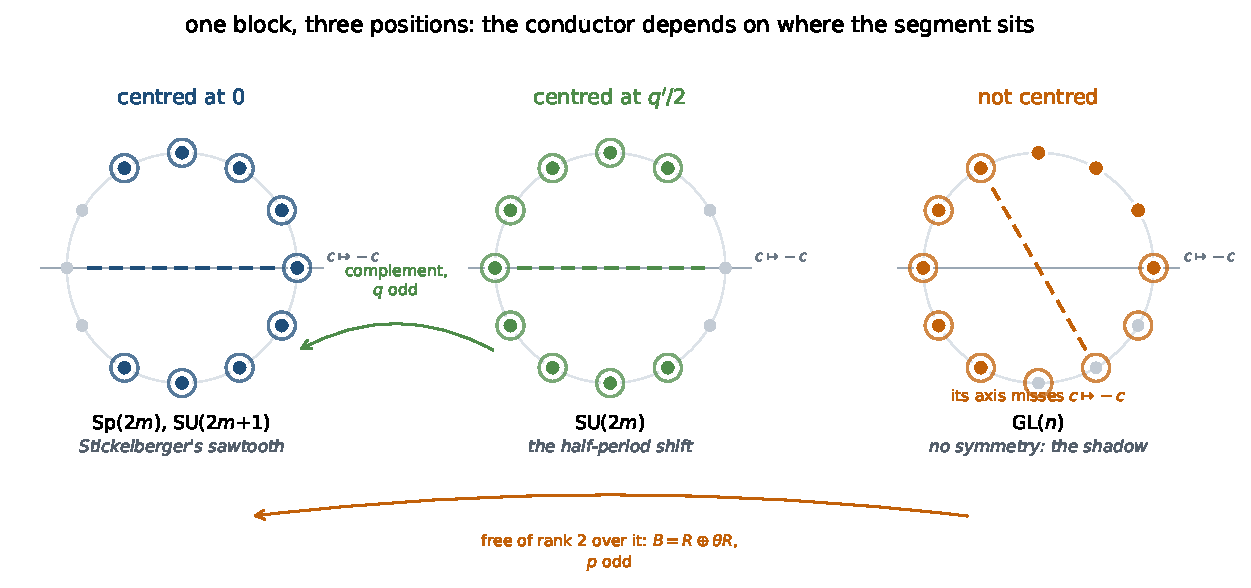
\includegraphics[width=\textwidth]{fig_formas.pdf}
\caption{The same block of residues, in the three positions the classical groups realise. Filled
dots are the classes the segment occupies; the hollow rings are their images under $c\mapsto-c$; the
dashed line is the block's own axis, through its midpoint. When the block is centred at $0$ or at
$q'/2$ that axis is the grey axis $c\mapsto-c$, the rings fall on the dots, and the ring of character
values is real; when it is not centred the two axes part, the rings come away from the dots, and the
ring is not real. The green arrow is Corollary~\ref{cor:par}: for $q$ odd the middle position is not
a separate regime, because the complement carries it to the left one. The orange arrow is
Theorem~\ref{obs:puente}, and it is weaker in kind: the right position does not \emph{become}
the left one, but locally at an odd $p$ and in the families $n=Nr,Nr+1$ it is a free extension of rank $2$ of
it, $B=R\oplus\theta R$, where $R$ is the ring of the segment recentred at $Nr/2$ --- a segment of
the leftmost kind. So the three positions are two, and the second sits over the first.}
\label{fig:formas}
\end{figure}

\pregunta{If the position of the block is what matters, which positions can produce a defect at
all, how large is it, and what decides its size?}

The table answers them, one row per section, and adds the answer the question did not ask for:
the uncentred position is not a regime of its own either, but sits over the first as a free
extension of degree $2$. As in \cite{Cond}, a statement is either proved or marked
\emph{measured} with the number of cells behind it; what is left open is marked
$\triangleright$ where it arises, and the two that outlive their own section are collected at
the end.

\begin{table}[tb]
\centering\small
\rowcolors{2}{filaclara}{white}
\begin{tabular}{@{}p{0.40\textwidth}p{0.55\textwidth}@{}}
\toprule
question & answer \\
\midrule
Why do two different groups give the same ring? (\S\ref{sec:seg}) &
because they give the same segment up to a monic integer factor: three operations, one division
lemma. The middle one is level-rank duality, known since \cite{PS86,NT92}; the other two are not,
and the same lemma proves all three. Lemma~\ref{lem:div},
Figure~\ref{fig:operaciones} \\
What does the defect look like at one prime? (\S\ref{sec:loc}) &
a single residue field, a first layer measured by a cyclic module, and
when $e=2$, $v_p=2\dim-1-W_1$: Theorem~\ref{thm:loc}, Figure~\ref{fig:plano} \\
Which primes can occur at all? (\S\ref{sec:sop}) &
only those with $r\mid n-1,n,n+1$: inside the families the defect is forced once
$\varphi(q')\ge4$ (Proposition~\ref{prop:conv}), outside them the order is maximal, by a lemma about intervals of
residues and a count of moments at the first layer: Lemma~\ref{lem:inter},
Proposition~\ref{prop:sop}, Theorem~\ref{thm:sop} \\
And when the segment is not centred? (\S\ref{sec:sombra}) &
the same picture with the layer dimension doubled, generators being twisted Gaussian binomials ---
and, in the families $n=Nr,Nr+1$ with $2\le n<q$, a free quadratic extension $B=R\oplus\theta R$ of the ring of
the recentred segment, its layers being those of $R$ added to themselves shifted by $P$ and its
type equal:
Lemma~\ref{lem:gauss}, Theorem~\ref{thm:sombra}, Theorem~\ref{obs:puente},
Proposition~\ref{prop:tipopuente}, Figure~\ref{fig:puente} \\
Why do class numbers appear? (\S\S\ref{sec:loc}, \ref{sec:sombra}) &
$h^-$ governs whether the first layer is full --- where the hypotheses of Theorem~\ref{thm:loc}
and Proposition~\ref{prop:capa1} hold, and only as a measurement in the even regime, $q$ even and
$p$ odd --- and in the shadow whether it reaches its reference rank $d+1$, with the
Euler factor at $2$ as a second source when the segment covers whole periods:
Theorem~\ref{thm:loc}, Proposition~\ref{prop:capa1}, Theorem~\ref{obs:puente} \\
\bottomrule
\end{tabular}
\end{table}

\section{The segment, and the three operations that preserve the ring}\label{sec:seg}

Write the eigenvalues of $g_q$ as $x_j=\zeta_M^{a_j}$. The multiset $\{a_j\}$ is the
\emph{segment}. For $\Sp(2m)$ at the principal element of type $\rho$ it is $\{\pm1,\dots,\pm m\}$
with $M=q$. For $\SU(n)$, with $\rho=\bigl(\tfrac{n-1}{2},\dots,-\tfrac{n-1}{2}\bigr)$, the entries
are integers when $n$ is odd and half-integers when $n$ is even, so
\[
\{-m,\dots,m\}\ \ (n=2m+1,\ M=q),\qquad
\{\pm1,\pm3,\dots,\pm(n-1)\}\ \ (n\ \text{even},\ M=2q).
\]
In both cases the segment is symmetric, so $g_q$ is conjugate to its inverse and every character
value is real; $A$ is an order in the real subfield. It is convenient to write both cases on the
same circle: with $t=\zeta_{2q}$ the segment of $\SU(n)$ is
\[
\marco{\{\,n-1,\ n-3,\ \dots,\ 1-n\,\}\subset\ZZ/2q ,}
\]
$n$ terms of one parity class modulo $2q$ --- so for $n$ even $g_q$ has order $2q$ in $\SU(n)$,
and order $q$ only in the adjoint group; we keep $q$ as the parameter --- and the characteristic
polynomial of $g_q$ in the standard representation is $F_{n,q}(T)=\prod_{j=0}^{n-1}\bigl(T-t^{\,n-1-2j}\bigr)$.

Since the fundamental characters of $\SU(n)$ are, up to a unipotent triangular change over $\ZZ$,
the elementary symmetric functions of the eigenvalues, and $e_n=\prod_jx_j=1$, the ring $A$ is
generated by the coefficients of $F_{n,q}$. Everything in this section is then a statement about
polynomials, and one lemma proves all of it.

\begin{lemma}[division]\label{lem:div}
For a monic $F\in\cO[T]$ let $\mathcal A(F)\subseteq\cO$ be the subring generated by its
coefficients. If $F,G$ are monic and $FG\in\ZZ[T]$, then $\mathcal A(F)=\mathcal A(G)$. In
particular, multiplying $F$ by a monic factor of $\ZZ[T]$ does not change $\mathcal A(F)$.
\end{lemma}

\begin{proof}
Dividing $FG\in\ZZ[T]$ by the monic $F$ is a division inside $\mathcal A(F)[T]$: the quotient, which
is $G$, has all its coefficients in $\mathcal A(F)$. Hence $\mathcal A(G)\subseteq\mathcal A(F)$,
and exchanging $F$ and $G$ gives the other inclusion. For the last sentence, if $H\in\ZZ[T]$ is
monic then $F$ and $FH$ have the same coefficient ring: $\mathcal A(FH)\subseteq\mathcal A(F)$ is
clear, and dividing $FH$ by the monic integer polynomial $H$ recovers $F$ inside
$\mathcal A(FH)[T]$.
\end{proof}

The three operations are three ways of supplying such a factor.

\begin{proposition}[the three operations]\label{prop:ops}
Fix $q$ and write $A_{\SU(n)}(q)$ for the ring generated by the character values of $\SU(n)$ at
$g_q$. Then
\begin{enumerate}
\item[(a)] \emph{adjoining an eigenvalue $1$:} $A_{\SU(2m+1)}(q)=A_{\Sp(2m)}(q)$;
\item[(b)] \emph{the complement:} $A_{\SU(n)}(q)=A_{\SU(q-n)}(q)$ for $1\le n<q$;
\item[(c)] \emph{the period:} $A_{\SU(n+q)}(q)=A_{\SU(n)}(q)$.
\end{enumerate}
\end{proposition}

\begin{proof}
(a) The segment of $\SU(2m+1)$ is that of $\Sp(2m)$ together with one extra eigenvalue equal to
$1$, so the two characteristic polynomials differ by the monic factor $T-1\in\ZZ[T]$, and
Lemma~\ref{lem:div} applies. (The generators of $\Sp(2m)$ are its own fundamental characters, again
a triangular change from the $e_k$ of its $2m$ eigenvalues.)

(b) The $q$ exponents $n-1-2j$, $0\le j\le q-1$, run over one full parity class modulo $2q$, so
\[
\marco{\prod_{j=0}^{q-1}\bigl(T-t^{\,n-1-2j}\bigr)=T^q-(-1)^{n-1}\in\ZZ[T].}
\]
The first $n$ factors are $F_{n,q}$. In the remaining $q-n$ the exponents are
$-(n+1)-2i$, $0\le i\le q-n-1$, which is the segment of $\SU(q-n)$ translated by $q$; translating by
$q$ multiplies every eigenvalue by $t^q=-1$, and $e_k(-x)=(-1)^ke_k(x)$, so that factor is
$(-1)^{q-n}F_{q-n,q}(-T)$ and has the same coefficient ring as $F_{q-n,q}$. Now apply
Lemma~\ref{lem:div}.

(c) The segment of $\SU(n+q)$ is one full parity class together with the segment of $\SU(n)$
translated by $q$; the first contributes the monic integer factor $T^q-(-1)^{n+q-1}$ and the second,
as in (b), has the coefficient ring of $\SU(n)$.
\end{proof}

\noindent Part (b) is not new, and its combinatorial reason is the one everybody uses: choosing $n$
of $q$ things is choosing the other $q-n$. With $q=n+k$ it is the level-rank pairing
$\SU(n)_k\leftrightarrow\SU(k)_n$. Witten derives it from
$G_V(k,N)\cong G_{V^*}(N-k,N)$ and attributes the $k\leftrightarrow N-k$ symmetry of loop group
representations to Pressley and Segal \cite[\S3]{Wit93}, \cite[Prop.~(10.6.4)]{PS86}; the explicit
relation between the modular matrices of $\widehat{\mathfrak{su}}(N)_K$ and
$\widehat{\mathfrak{su}}(K)_N$ is \cite[(3.8)]{NS07}, whose row $R'=0$ says that the quantum
dimensions agree; Naculich and Schnitzer attribute it to earlier work
\cite{ABI90,SA91,MNRS91}, and the proof for WZW models is \cite{NT92}. What (b) adds is the formulation as an equality
of \emph{orders} --- that literature asks about fusion algebras and quantum dimensions, not about
the ring the values generate --- and a proof that is three lines of polynomial algebra, with no
fusion category, no modular matrices and no loop group. The same three lines give (a) and (c),
which are not level-rank.

\medido{Not the ring but the \emph{values}: computing $\chi_\lambda(g_q)$ by the bialternant in
$\QQ(\zeta_{2q})$ over the whole alcove, the sets of character values of $\SU(n)$ and of
$\SU(q-n)$ at $g_q$ coincide exactly --- not merely up to sign --- in $25$ of $25$ pairs with
$q\le12$, up to $462$ values a side. That is sharper than the equality of rings, and it is what
identifies (b) with level-rank rather than merely with something like it. For the normalised quantum
dimensions the row $R'=0$ of \cite[(3.8)]{NS07} already gives it; the measurement is a control of
our conventions, not a substitute for that proof.}

\begin{figure}[htbp]
\centering
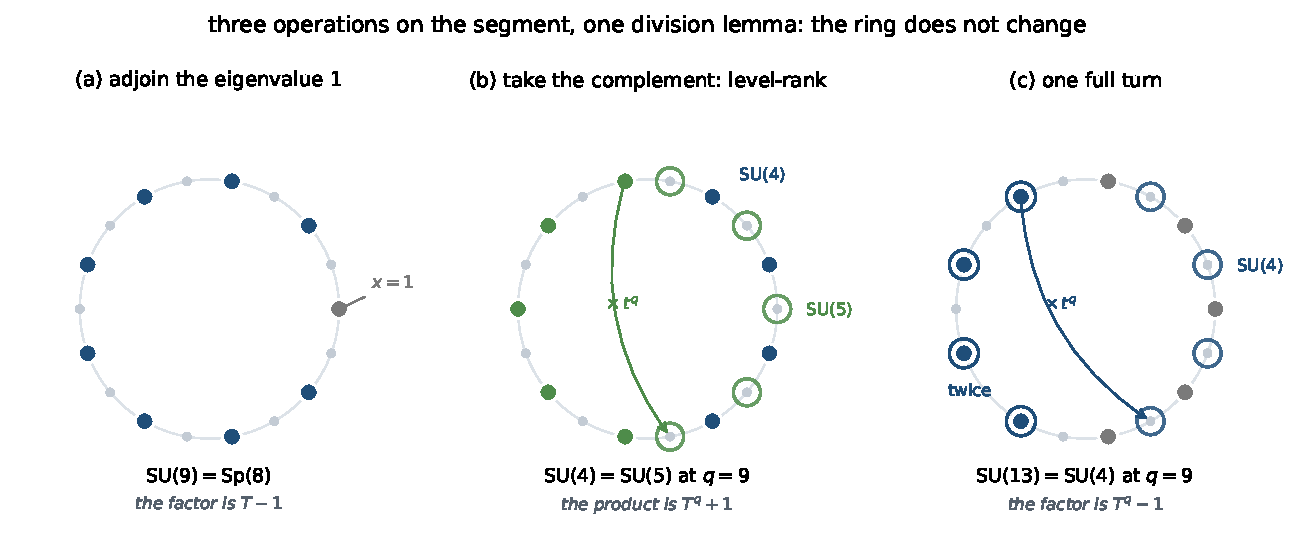
\includegraphics[width=\textwidth]{fig_operaciones.pdf}
\caption{The three operations of Proposition~\ref{prop:ops} on the circle of $2q$-th roots of unity,
drawn at $q=9$. The segment of $\SU(n)$ is $n$ consecutive exponents of one parity class. (a)
Adjoining the eigenvalue $1$ is the factor $T-1$. (b) The $n$ exponents and the remaining $q-n$
multiply to $T^q+1$, and the leftovers are the segment of $\SU(q-n)$ turned half a turn, which is
multiplication by $t^q=-1$; this panel is level-rank duality, and the half turn is all that the
division lemma has to absorb. (c) Thirteen exponents at $q=9$ cover the class once and four of them
twice; the full class is the factor $T^q-1$ and the four that repeat are again $\SU(4)$ up to
$t^q$.}
\label{fig:operaciones}
\end{figure}

\medido{$287$ cells with $m\le7$, $q\le49$ for (a), comparing the two \emph{lattices} and not merely
their indices; $90$ complements and $82$ periods, also as lattices, with $q\le21$ and
$\varphi(2q)\le24$. No discrepancy.}

Two consequences deserve to be stated separately, because they remove a case rather than add one.

\begin{corollary}\label{cor:par}
Let $q$ be odd and $n<q$ even. Then $A_{\SU(n)}(q)=A_{\Sp(q-n-1)}(q)$; for $n>q$ apply
Proposition~\ref{prop:ops}(c) first.
\end{corollary}

\begin{proof}
$q-n$ is odd, so Proposition~\ref{prop:ops}(b) and then (a) apply.
\end{proof}

So for $q$ odd the even case is not a separate theory: it is the type-$C$ ring at the same $q$, on
the nose and not merely up to conjugacy. What survives of \S\ref{sec:par} is the case $q$ even.

\begin{remark}[the even segment is $\Sp(2m)$ at the other principal element]
The segment $\{\pm1,\pm3,\dots,\pm(2m-1)\}$ of $\SU(2m)$ is also the segment of $\Sp(2m)$ at
$\exp(2\pi i\rho^\vee/q)$, since $\rho^\vee=(m-\tfrac12,\dots,\tfrac12)$ for $C_m$ gives exactly the
odd exponents modulo $2q$. As the spectrum is inverse-closed, the $e_k$ of $\Sp$ and of $\SU(2m)$
generate the same ring. The two principal elements $\rho$ and $\rho^\vee$ of $\Sp(2m)$ are therefore
the two symmetric positions of Figure~\ref{fig:formas}, and type $A$ adds no third one.
\end{remark}

\begin{remark}[why $\Sp$ had to appear]
The pair $(\SU(2m+1),\Sp(2m))$ is the folding $A_{2m}\rightsquigarrow C_m$: the fixed group of the
diagram automorphism of $\SL(2m+1)$ is $\SO(2m+1)$, whose dual is $\Sp(2m)$; and $g_q$, having
inverse-closed spectrum and determinant~$1$, lies up to conjugacy in that fixed group. Jantzen's
twining character formula \cite{Jan,Hopper,FSS} lives in the same picture, but it equates a
\emph{twisted} trace with an ordinary character of the dual of the fixed group, whereas
Proposition~\ref{prop:ops}(a) equates ordinary values with ordinary values and is proved by a
division. We cite it as context, not as precedent.
\end{remark}

\section{The local picture}\label{sec:loc}

Fix $p$ and write $M=p^vq'$ with $p\nmid q'$, $E=\varphi(p^v)$, $d=\varphi(q')/2$. We assume
$n\not\equiv0,\pm1\pmod q$, since otherwise $A=\ZZ$ by Proposition~\ref{prop:ops} and there is
nothing to compute, and $q'\ge3$: for $q'\le2$ the residual algebra is $\FF_p$, $d$ must be read
as $1$, and the matrix of Theorem~\ref{thm:loc}(b) has no columns --- at $\SU(3)$, $q=8$, $p=2$
it has rank $0$ while $W_1=1$. In
$\ZZ_p[\zeta_M]$ write $\zeta_M=\omega\rho$ with $\omega$ of order $q'$ and $\rho$ of order $p^v$,
and put $\pi=\rho-1$, a uniformiser, $\gamma_c=\omega^c$, and
\[
N_c=\#\{j:a_j\equiv c\ (q')\},\qquad S(c)=\sum_{a_j\equiv c}a_j .
\]
By the symmetry of the segment $S(-c)=-S(c)$; in particular $S(0)=0$, and $S(q'/2)=0$ when $q'$ is
even.

\begin{lemma}[first order]\label{lem:orden1}
With $F(T)=\prod_c(T-\gamma_c)^{N_c}$,
\[
\marco{\prod_j(T-x_j)\;=\;F(T)\;-\;\pi\sum_c S(c)\,\gamma_c\,\frac{F(T)}{T-\gamma_c}\;+\;O(\pi^2).}
\]
\end{lemma}

\begin{proof}
Since $\rho=1+\pi$, each eigenvalue is
$x_j=\omega^{a_j}\rho^{a_j}=\gamma_{a_j}\bigl(1+a_j\pi+O(\pi^2)\bigr)$, so
$T-x_j=(T-\gamma_{a_j})-a_j\gamma_{a_j}\pi+O(\pi^2)$. Expanding the product over $j$ and keeping the
term linear in $\pi$,
\[
\prod_j(T-x_j)=\prod_j(T-\gamma_{a_j})-\pi\sum_j a_j\gamma_{a_j}\prod_{i\neq j}(T-\gamma_{a_i})+O(\pi^2),
\]
and $\prod_{i\neq j}(T-\gamma_{a_i})=F(T)/(T-\gamma_{a_j})$, an exact division in $\cO[T]$. Grouping
the indices $j$ by the class $c=a_j\bmod q'$ turns $\sum_j a_j\gamma_{a_j}F(T)/(T-\gamma_{a_j})$ into
$\sum_c S(c)\gamma_c F(T)/(T-\gamma_c)$.
\end{proof}

The lemma says that the first-order parts of \emph{all} the generators at once are the coefficients
of a single polynomial. They are not independent data: in the stable case (Definition~\ref{def:est}) --- residue scalar
and $E\ge2$, the setting of Theorems~\ref{thm:loc} and~\ref{thm:sombra} --- $\gr_1(A)$ is their
$\FF_p$-span; without stability the residual algebra multiplies them, and at $\GL(2)$, $q=15$,
$p=3$ they span one direction over $\FF_3$ while the layer is full, of dimension $4$. It is stated in
the eigenvalues $x_j$, which is the right model for the non-real ring of \S\ref{sec:sombra}; for a
symmetric segment one has to pass to real coordinates first, and that is where the quantum integers
of \cite{Cond} come from.

\begin{lemma}[real coordinates]\label{lem:real}
Let the segment be symmetric and write $\eta_j=x_j+x_j^{-1}$, $z=(\omega-\omega^{-1})\pi$ and
\[
U_c=\frac{\omega^c-\omega^{-c}}{\omega-\omega^{-1}},
\]
the quantum integer, which satisfies $\sigma_u(U_c)=U_{uc}/U_u$ and vanishes exactly when
$2c\equiv0$. Write also $\bar\gamma_c=\gamma_c+\gamma_c^{-1}$, the real counterpart of $\gamma_c$,
which still satisfies $\sigma_u(\bar\gamma_c)=\bar\gamma_{uc}$. Then $A=\ZZ[e_k(\eta)]$, each
$\eta_j\equiv\bar\gamma_{a_j}+a_jU_{a_j}z$ modulo $\rad^2$, and
\[
\marco{\prod_j(T-\eta_j)\equiv F_\eta(T)-z\,G(T),\qquad
G(T)=\sum_c S(c)\,U_c\,\frac{F_\eta(T)}{T-\bar\gamma_c},}
\]
where $c$ runs over one representative of each pair $\{c,-c\}$ of classes met by the half
segment, both in the sum and in $F_\eta=\prod_c(T-\bar\gamma_c)^{N_c}$, and $N_c$ counts the
$a_j>0$ with $a_j\equiv\pm c$. Summing $S(c)U_c$ over both members of a pair would count each term
twice, since $S(-c)=-S(c)$ and $U_{-c}=-U_c$.
\end{lemma}

\begin{proof}
For a symmetric segment $\prod_j(T-x_j)=(T-1)^{\varepsilon}\prod_{j>0}(T^2-\eta_jT+1)$ with
$\varepsilon\in\{0,1\}$. The factor $(T-1)^\varepsilon$ is monic in $\ZZ[T]$, so by
Lemma~\ref{lem:div} it may be dropped; and the coefficients of the remaining product are
$\ZZ$-polynomials in the $e_k(\eta)$, triangularly, and conversely, so the ring is
$\ZZ[e_k(\eta)]$. The expansion is Lemma~\ref{lem:orden1} applied to the $\eta_j$: from
$x_j=\gamma_{a_j}(1+a_j\pi+O(\pi^2))$,
\[
\eta_j=\gamma_{a_j}+\gamma_{a_j}^{-1}+a_j\pi(\gamma_{a_j}-\gamma_{a_j}^{-1})+O(\pi^2)
=\bar\gamma_{a_j}+a_jU_{a_j}z+O(\pi^2),
\]
and grouping the $j>0$ by pairs $\{c,-c\}$, whose terms $a_jU_{a_j}$ add up to $S(c)U_c$, gives
$G$. Note that $z$, not $\pi$, is the uniformiser of the real ring --- up to a term of order $\pi^2$:
$z$ itself is not real, its conjugate being $z/(1+\pi)$, and the real element
$z_0=\zeta_M+\zeta_M^{-1}-(\omega+\omega^{-1})$ agrees with it modulo $\pi^2$, which is all that
is used. The two differ by the unit $\omega-\omega^{-1}$, and it is exactly that unit which turns the
non-real coefficient $\gamma_c$ of Lemma~\ref{lem:orden1} into the real $U_c$. Writing $G$ with
$\gamma_c$ in place of $U_c$, or with $T-\gamma_c$ in place of $T-\bar\gamma_c$, would be a
different polynomial: the two models must not be mixed.
\end{proof}

\begin{definition}\label{def:est}
The segment is \emph{stable} at $q'$ if the multiset $\{a_j\bmod q'\}$ is invariant under
multiplication by every unit of $\ZZ/q'$.
\end{definition}

\begin{lemma}\label{lem:est}
The segment is stable at $q'$ if and only if $N_c$ depends only on $\gcd(c,q')$.
\end{lemma}

\begin{proof}
The orbits of $(\ZZ/q')^\times$ on $\ZZ/q'$ are the sets $\{c:\gcd(c,q')=D\}$, one for each divisor
$D$ of $q'$. A multiset is invariant exactly when its multiplicity function is constant on orbits.
\end{proof}

We write $\rad$ for the radical of $\cO_p=\cO\otimes\ZZ_p$ (for the real ring, of the real
$\cO_p$), $\bar R=\cO_p/\rad$ for the residual algebra, of dimension $d$ over $\FF_p$, and
$W_i=\dim_{\FF_p}\bigl((A_p\cap\rad^i)+\rad^{i+1}\bigr)/\rad^{i+1}$ for the dimension of the
$i$-th layer of $A$; $e$ is the least $i$ with $A_p\supseteq\rad^i$, the exponent of the
conductor.

\begin{theorem}[local structure; {\cite[Thm.~5]{Cond}}]\label{thm:loc}
Assume the segment is stable at $q'$ and $E\ge2$. Then
\begin{enumerate}
\item[(a)] $F_\eta\in\FF_p[T]$, the image of $A$ in $\bar R$ is $\FF_p$ --- that is, $W_0=1$ --- and $A$
has a single maximal ideal above $p$, with residue field $\FF_p$;
\item[(b)] $W_1=\dim_{\FF_p}\FF_p[(\ZZ/q')^\times]\cdot S$, the rank modulo $p$ of
$[S(u^{-1}c)]$ with rows $u\in(\ZZ/q')^\times/\pm1$ and columns the classes with $2c\not\equiv0$;
\item[(c)] if moreover $d\ge2$, then $e=1$ if and only if $W_1=d$;
\item[(d)] $v_p([\cO:A])=\sum_{i<e}(d-W_i)$; in particular $v_p=d-1$ when $e=1$ and
$v_p=2d-1-W_1$ when $e=2$.
\end{enumerate}
\end{theorem}

\begin{proof}
(a) Stability makes the Galois group permute the factors of $F_\eta$, so its coefficients are fixed
and $F_\eta\in\FF_p[T]$; the $e_k$ reduce to those constants in every residue field.

(b) Every element of $A$ is $\Phi(e)$ with $\Phi\in\ZZ[X]$, and modulo $\rad^2$,
\[
\Phi(e)\;\equiv\;\Phi(F_\eta)+z\sum_k(\partial_k\Phi)(F_\eta)\,G_k ,
\]
with $\Phi(F_\eta)\in\FF_p$ and $p\in\rad^2$ because $E\ge2$. So $\gr_1(A)$ is the $\FF_p$-span $V$ of
the coefficients $G_k$, which by Lemma~\ref{lem:real} are those of $G$.
As $\bar R$ is \'etale, $\bar R\otimes\overline{\FF}_p\cong\overline{\FF}_p^{\,d}$ through the
embeddings $\sigma_u$, and extension of scalars is injective on $\FF_p$-subspaces, so $\dim V$ is
the rank of the matrix whose row $u$ lists the coefficients of $\sigma_u(G)$. From
$\sigma_u(\bar\gamma_c)=\bar\gamma_{uc}$, $\sigma_u(U_c)=U_{uc}/U_u$ and the stability of
$F_\eta$,
\[
U_u\,\sigma_u(G)=\sum_c S(u^{-1}c)\,U_c\,\frac{F_\eta(T)}{T-\bar\gamma_c},
\]
and multiplying a row by the unit $U_u$ does not change the rank; the functions
$U_cF_\eta/(T-\bar\gamma_c)$, one for each class $c$ up to sign, are independent and do not depend
on $u$ --- the classes $c$ and $-c$ give opposite functions and columns that agree up to sign, so
keeping both does not change the rank --- and the classes with $2c\equiv0$ contribute nothing
because there $U_c=0$ (and $S(c)=0$).

(c) If $\gr_1(A)=\gr_1(\cO)$ then $\gr_i(A)\supseteq\gr_1(A)^i=\gr_i(\cO)$ for all $i$, since
$\gr(\cO_p)$ is a polynomial ring over $\bar R$, and the filtration collapses, so $e\le1$; and
$e\ge1$ because $W_0=1<d$ makes $A_p\ne\cO_p$. The converse is clear.

(d) Filter $\cO_p$ and $A_p$ by $\rad^i$; for $i\ge e$ one has $A_p\cap\rad^i=\rad^i$, so only the
layers $i<e$ contribute, with quotients of dimension $d-W_i$. The layer $i=0$ always contributes
$d-1$, by (a).
\end{proof}

\medido{The instrument reproduces the published type-$C$ law in $18$ of $18$ cells. In type $A$,
(d) with $e=2$ holds in $44$ of $44$ cells under $W_1>d/2$; of the $18$ cells outside the
hypothesis, $15$ still agree and the $3$ that fail all have $W_1=0$, the ladder zone of
\cite{Cond}. Statement (b) holds in
$193$ of $193$ stable cells and in $98$ of $127$ unstable ones: the hypothesis is not decoration.
That $W_0=1$ is not assumed but read off the instrument in every cell tabulated in
\S\ref{sec:sop}.}

The last clause of (d) is worth saying out loud, because it is what \S\ref{sec:sop} rests on: under
the hypotheses of the theorem the defect is never zero once $d\ge2$. A full first layer makes $e=1$,
not $v_p=0$.

That $d\ge2$ is not decoration either, and it is why (c) carries it while the other three parts do
not. At $\SU(3)$ with $q=12$ and $p=3$ the segment $\{1,0,-1\}$ is stable at $q'=4$ with $E=2$, and
$d=1$, so $W_1=1=d$ --- and yet $A=\ZZ[\sqrt3]=\cO$ is maximal, $\mathfrak f=\cO$ and $e=0$. What
fails is not the layer count but the step before it: $W_0=1$ stops forcing a defect once $d=1$, and
then $e=1$ has nothing to be. Parts (a), (b) and (d) stand as written, (d) reading as the empty sum.
The source keeps the same corner out by excluding $q'\in\{1,2,3,4,6\}$ among its standing hypotheses
\cite[\S5]{Cond}.

Statement (d) is a plane, and it is worth seeing it as one. Over a wider sweep of $417$ cells the
real ring lives with $d=\varphi(q')/2$ and the shadow of \S\ref{sec:sombra} with $D=\varphi(q')$; if
the layer dimension is put on an axis, \emph{both} populations lie on the same plane
$v=2\dim-1-W_1$. That is the thesis of this note in one picture: the group does not enter, only the
segment does.

The plane is the face $e=2$ of (d), and it is worth knowing what lies off it. In the regime of
Theorem~\ref{obs:puente} with $p\nmid N$ and the real profile of \cite{Cond} (the display after
Proposition~\ref{prop:tau}), writing $\delta=d-W_1(R)$ for the drop of the real first layer, the
shadow has $W_1=d+1-\delta$ and $\dim=2d$, so the plane would
predict $3d-2+\delta$ while the true index is $3d-2+2\delta$: a cell of the shadow sits
\emph{exactly $\delta$ above the plane}, and the height off the plane is the class-number defect.
With $p\mid N$ the count is different: at $q=45$, $p=3$, $N=3$ the shadow has $W_1=0$ and
$v_3([\cO:B])=14$, where this reading would give $1$ and $8$.
No cell of the sweep shows this --- its $14$ off-plane shadow cells all have $p=2$ or
$(p,q')=(3,4)$, outside that regime, and the sweep never reaches the first conductor with
$\delta>0$ --- so the figure is a picture of the face $\delta=0$.

\begin{figure}[htbp]
\centering
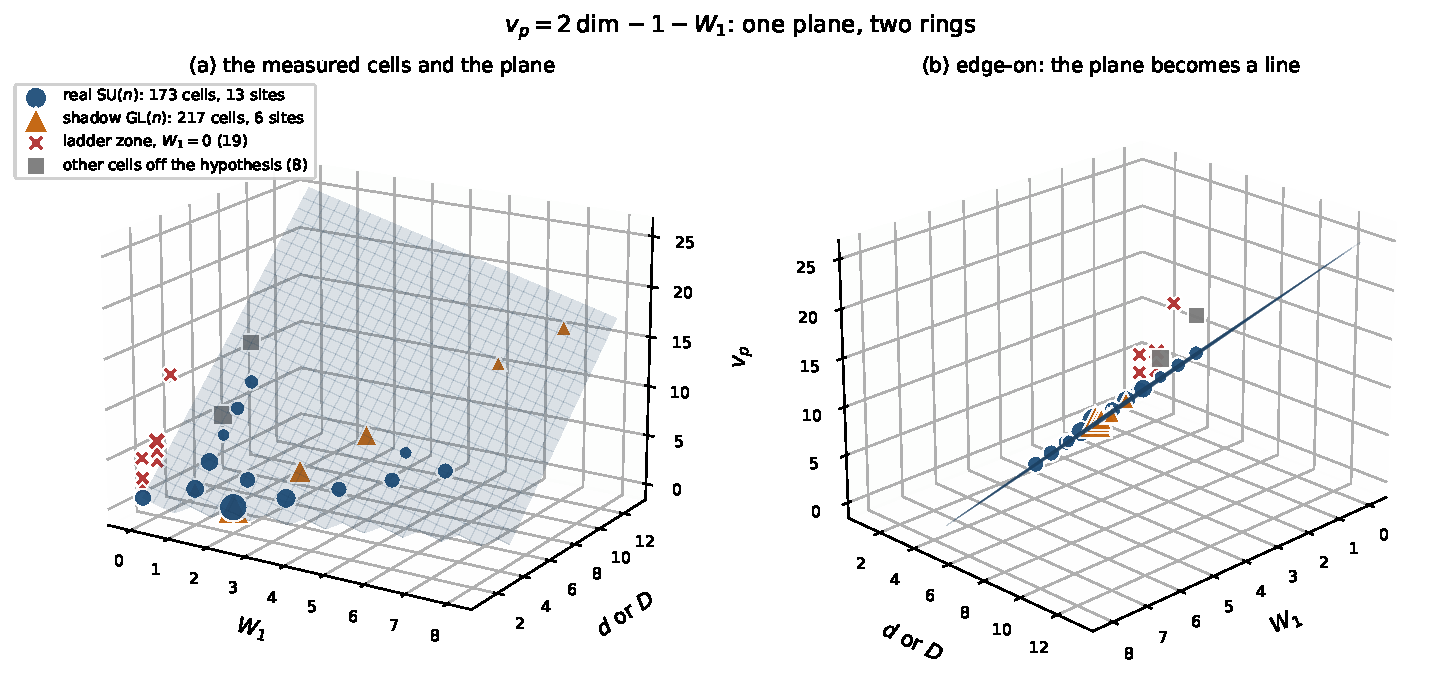
\includegraphics[width=\textwidth]{fig_plano.pdf}
\caption{Each measured cell is a point $(W_1,\dim,v_p)$; many cells share a position, and the size
of a marker says how many. \emph{Left}: the cells and the plane. \emph{Right}: seen along
$(1,1,1)$, which is orthogonal to the normal $(1,-2,1)$, the plane projects to a line and whatever
lies on it becomes collinear. Under the hypothesis $W_1>\dim/2$ all $335$ cells lie on the plane;
the $27$ that do not are shown apart, $19$ of them in the ladder zone $W_1=0$. All $14$ off-plane
cells of the shadow have $p=2$ or $(p,q')=(3,4)$; none is in the regime of
Theorem~\ref{obs:puente}, where the shadow leaves the plane upwards by exactly $\delta$.}
\label{fig:plano}
\end{figure}

\section{Support: which primes can occur}\label{sec:sop}

Throughout this section write
\[
r=\frac{q}{p^{v_p(q)}},
\]
the prime-to-$p$ part of $q$ --- not of $M$. For $n$ odd, and for $n$ even with $p=2$, one has
$r=q'$. For $n$ even and $p$ odd, $M=2q$ gives $q'=2r$: the segment then occupies the odd residues
modulo $2r$, which as an arithmetic progression has period $r$, and $r$ is the modulus that the
criterion sees.

\begin{proposition}\label{prop:fam}
If $r$ divides $n-1$, $n$ or $n+1$, then the segment of $\SU(n)$ is stable at $q'$.
\end{proposition}

\begin{proof}
By Lemma~\ref{lem:est} it suffices to see that $N$ is constant on the orbits of $(\ZZ/q')^\times$.
There are three branches. For $n$ odd, $M=q$ and $q'=r$, and the segment $\{-m,\dots,m\}$ is $n$
consecutive residues of $\ZZ/r$. For $n$ even it is the progression $\pm1,\pm3,\dots,\pm(n-1)$ of
difference $2$ modulo $M=2q$: with $p=2$ one has $q'=r$ odd and the difference is invertible, and
with $p$ odd one has $q'=2r$ and the progression runs through the odd classes, returning to the start
after $r$ steps. In every branch the progression has period $r$, so the classes it does not meet are
either none or all the even ones, and those are permuted among themselves by the units, so they
contribute nothing. On the classes it meets, $N_c\in\{\lfloor n/r\rfloor,\lceil n/r\rceil\}$, and
the two values coincide when $r\mid n$. If $n\equiv\pm1\pmod r$, exactly one class $c$ is off by
one, and since the segment is symmetric $N_{-c}=N_c$, so that class satisfies $c\equiv-c$. Such a
class is fixed by every unit, because the orbit of $c$ has $\varphi(q'/\gcd(c,q'))$ elements and
that is $1$ exactly when $2c\equiv0$. So $N$ is constant on orbits. (For $n$ odd the exceptional
class is not always the centre $0$: writing $n=Ar\pm1$ it is $Ar/2\bmod r$, which is $q'/2$ when
$A$ is odd --- at $\SU(5)$ with $q'=4$ it is $2$.)
\end{proof}

\medido{$807$ cells with $n\le25$, $q\le60$, over the four branches (both parities of $n$ and of
$r$): every cell in a family is stable, with no exception.}

The converse fails: there are stable segments outside the families, the smallest being $n=3$,
$q'=6$, whose residues $\{0,1,5\}$ are the union of the orbits $\{0\}$ and $\{1,5\}$. Every one of them
has $q'=6$, as Lemma~\ref{lem:inter} will force, and they are maximal for the reason given in the
proof of Proposition~\ref{prop:sop}: there $d=1$ and $W_1=1$. It is not $d=1$ alone: inside the
families, $d=1$ can carry a defect.

Inside the families the defect is not merely possible: it is forced, and by the local law itself.

\begin{proposition}[the families always give a defect]\label{prop:conv}
Let $E\ge2$, let the segment be stable at $q'$ --- by Proposition~\ref{prop:fam} it is enough that
$r$ divide one of $n-1,n,n+1$ --- and let $\varphi(q')\ge4$, that is $q'\notin\{1,2,3,4,6\}$,
that is $d\ge2$. Then
\[
\marco{p\mid[\cO:A],\qquad\text{indeed } v_p([\cO:A])\ \ge\ d-1 .}
\]
\end{proposition}

\begin{proof}
Theorem~\ref{thm:loc} applies. By (a) the layer $i=0$ contributes $d-W_0=d-1$ to the sum in (d),
and every term of that sum is $\ge0$.
\end{proof}

So inside the families a defect can be avoided only in the range $\varphi(q')\le2$, where $d=1$
and the argument says nothing: the layer $i=0$ is then full by default, and a defect, if there is
one, sits in the deeper layers. It can: $\SU(11)$ at $q=36$ and $p=3$ is in the family $r=4\mid12$,
has $d=1$, and has index $3$, with profile $(1,0,1,\dots)$.

\medido{$26$ of $26$ stable cells with $E\ge2$ and $d\ge2$, over $n\le7$ and $q\le40$, have
$v_p\ge d-1$; restricted to the cells in a family with $r\notin\{1,2,3,4,6\}$, $23$ of $23$ have
$p\mid[\cO:A]$.}

\begin{lemma}[stable intervals]\label{lem:inter}
Let $q'\ge3$ and let $I\subseteq\ZZ/q'$ be a set of $B$ consecutive residues with $2\le B\le q'-2$.
If $\alpha(I)=I$ for one affine bijection $\alpha(x)=ux+b$ of $\ZZ/q'$, then $u\equiv\pm1\pmod{q'}$.
In particular, if $I$ is a union of the
strata $X_D=\{c:\gcd(c,q')=D\}$ then $\varphi(q')\le2$; indeed the only such $I$ occur at $q'=6$,
$B=3$, and they are $\{5,0,1\}=X_1\cup X_6$ and $\{2,3,4\}=X_2\cup X_3$.
\end{lemma}

\begin{proof}
The complement of a proper cyclic interval is a cyclic interval, and it is $\alpha$-stable when $I$
is; so we may replace $I$ by the shorter of the two, an interval $J$ of length $b$ with
$2\le b\le q'/2$ and $\alpha(J)=J$. Put $C_J(t)=|J\cap(J+t)|$. The bijection $\alpha$ carries
$J\cap(J+t)$ onto $\alpha(J)\cap(\alpha(J)+ut)=J\cap(J+ut)$, so $C_J(ut)=C_J(t)$, and in
particular $C_J(u)=C_J(1)=b-1$. On the other hand $C_J$ does not change when $J$ is translated, and for
$J=\{0,\dots,b-1\}$ and $1\le t<q'$
\[
C_J(t)=\max(0,b-t)+\max(0,b-(q'-t)).
\]
Since $2b\le q'$ the two terms are never positive together, and $b-1\ge1$; so $C_J(t)=b-1$
exactly when $t=1$ or $t=q'-1$, and $u\equiv\pm1$.

If $I$ is a union of strata it is stable under every unit, because multiplying by a unit does not
change $\gcd(c,q')$. So every unit is $\pm1$, that is $\varphi(q')\le2$ and $q'\in\{3,4,6\}$. At
$q'=3$ the range of $B$ is empty. Writing $I=\{a,\dots,a+B-1\}$, stability under $-1$ reads
$2a+B-1\equiv0\pmod{q'}$, which for $q'$ even forces $B$ odd: that excludes $q'=4$, where $B=2$,
and leaves $q'=6$, $B=3$, $a\in\{2,5\}$.
\end{proof}

\medido{The strong form by brute force: for every $q'\le120$, every interval with
$2\le B\le q'-2$ and every unit $u$, $uI=I$ only for $u=\pm1$ ($3.1\times10^7$ checks), and the
affine form for $q'\le60$ and every translation $b$ ($1.9\times10^6$ checks); and over
all $q'\le150$, all $B$ and all rotations, the only interval that is a union of strata outside
$B\in\{0,1,q'-1\}$ is one of the two at $q'=6$. The bound $B\ge2$ is not decoration: the singleton
$\{0\}$ is stable under every unit. That is the same $q'=6$ as in the cells recorded below.}

\begin{proposition}[support]\label{prop:sop}
Suppose $r$ divides none of $n-1$, $n$, $n+1$. Then either the segment is stable at $q'$, and then
$q'=r=6$ and $A$ is maximal at $p$; or it is not, and then the image of $A$ in $\bar R$ is all of
$\bar R$, that is $W_0=d$, and $A$ is maximal at $p$ when $v=0$.
\end{proposition}

\begin{proof}
Suppose $r$ divides none of the three. As in the proof of Proposition~\ref{prop:fam}, write the
segment in order as $a_j=a_0+\beta j$, $0\le j<n$, with $\beta=1$ for $n$ odd and $\beta=2$ for
$n$ even; the class of $a_j$ modulo $q'$ depends on $j$ only modulo $r$. Writing $n=Ar+B$, the
multiplicity is $A+1$ on the classes of the positions $J=\{0,\dots,B-1\}\subseteq\ZZ/r$ and $A$ on
the others, and $B\notin\{0,1,r-1\}$, so $2\le B\le r-2$. A unit $u$ of $\ZZ/q'$ sends $a_j$ to
$a_0+\beta\bigl(uj+(u-1)a_0/\beta\bigr)$ --- for $\beta=2$ the number $a_0$ is odd and $u$ is
odd --- so on positions it acts as the affine bijection $\alpha_u(j)=uj+(u-1)a_0/\beta$ of
$\ZZ/r$. The map $u\mapsto\alpha_u$ is injective: $u$ is determined by $u\bmod r$ unless $q'=2r$
with $r$ even, and then $u$ and $u+r$ differ by the translation $r/2$.

If $v=0$ the prime is unramified and $\cO_p/p\cO_p=\bar R$, so both cases below, which end with a
full residual image, give $A_p=\cO_p$ by Nakayama with no frontier. Suppose the segment stable at
$q'$. Then $\alpha_u(J)=J$ for every unit, and
Lemma~\ref{lem:inter} gives $u\equiv\pm1\pmod r$. An affine map with linear part $1$ fixes the
proper interval $J$ only if it is the identity, since $C_J(t)<C_J(0)$ for $t\ne0$, and one with
linear part $-1$ is then determined by $J$; so the units give at most two maps, and
$\varphi(q')\le2$. With $r\ge4$, forced by $2\le B\le r-2$, and $q'\in\{r,2r\}$ this leaves
$q'=r\in\{4,6\}$; $q'=r$ even means $n$ odd, and at $r=4$ that forces $B$ odd, outside $[2,2]$. So
$q'=r=6$, so $n$ is odd, $B=3$ and $n=6A+3$; and $p\ge5$, so $E\ge4$ when $v\ge1$. There $d=1$ and
the residual image is all of $\bar R=\FF_p$, which settles $v=0$. For $v\ge1$ the residue ring
$\bar R$ is $\FF_p$, and $\cO_p$ is a discrete valuation ring totally ramified over $\ZZ_p$: it is
generated over $\ZZ_p$ by any element of valuation one, so $A_p=\cO_p$ as soon as $W_1=1$. By
Theorem~\ref{thm:loc}(b), $W_1$ is the rank of the single row $(S(1),S(2),-S(2),-S(1))$ over the
classes $1,2,4,5$, and summing over $\{-m,\dots,m\}$ gives $(S(1),S(2))=(A+1,-A)$ for $A$ even and
$(A,-(A+1))$ for $A$ odd. Two consecutive integers are not both divisible by $p$; so $W_1=1$ and
there is no defect.

Otherwise the segment is unstable at $q'$, and more is true: by the same two steps a unit that fixes
the multiset gives an $\alpha_u$ fixing $J$, hence $u\equiv\pm1$ and $\alpha_u$ is one of at most two
maps, so the stabiliser of the multiset in $(\ZZ/q')^\times/\pm1$ is trivial. Then the image of
$A$ in $\bar R$ is all of $\bar R$, that is $W_0=d$: that image is generated by the coefficients of
$F_\eta$, and after extending scalars $\bar R\otimes\overline\FF_p\cong\overline\FF_p^{\,d}$
through the embeddings $\sigma_u$, a coefficient becomes the function
$u\mapsto$ (that coefficient of $\sigma_u(F_\eta)$). As the $\bar\gamma_c$ are distinct for
classes $c\not\equiv\pm c'$, two embeddings give the same polynomial only if $u'u^{-1}$ fixes the
multiset, so these functions separate the $d$ points, and functions separating the points of a
finite set generate all functions on it.
\end{proof}

A full residual image does not by itself make the order maximal: the index law of
Theorem~\ref{thm:loc} reads $v_p([\cO:A])=\sum_{i<e}(d-W_i)$, and $W_0=d$ kills the term $i=0$ and
no other. What closes the gap is that, once the residue field is reached, the first layer decides
everything, and the first layer is read off the moments.

\begin{proposition}[the first layer decides]\label{prop:tangente}
Let $E\ge2$ and suppose the image of $A$ in $\bar R$ is all of $\bar R$. Then $A_p=\cO_p$ if and
only if $p\nmid S(c)$ for some class $c$, taken with $2c\not\equiv0$ when the segment is symmetric.
\end{proposition}

\begin{proof}
The graded ring $\gr(A)$ is a graded subring of $\gr(\cO_p)=\bar R[\bar\varpi]$, polynomial in the
class of a uniformiser, and $\gr_0(A)=\bar R$ by hypothesis. So $\gr_1(A)$ is an $\bar R$-submodule
of $\gr_1(\cO_p)=\bar R\,\bar\varpi$ and $\gr_i(A)\supseteq\gr_1(A)^i$: if $\gr_1(A)=\gr_1(\cO_p)$
every layer is full and $A_p=\cO_p$, and conversely a maximal order has $W_1=d$. It remains to
identify $\gr_1(A)$. Each generator is $e_k=e_k^{(0)}+g_k\varpi+O(\varpi^2)$, where $e_k^{(0)}$ is
the corresponding coefficient of $F$ (or $F_\eta$), which lies in the unramified subring
$\ZZ_p[\omega]$, and $g_k$ is the corresponding coefficient of $G$ in Lemma~\ref{lem:orden1} (or
Lemma~\ref{lem:real}). An element $\Phi(e)$, $\Phi\in\ZZ_p[X]$, lies in $\rad$ exactly when
$\Phi(\bar e)=0$ in $\bar R$; then $\Phi(e^{(0)})\in\rad\cap\ZZ_p[\omega]=p\,\ZZ_p[\omega]
\subseteq\rad^E\subseteq\rad^2$, so the image of $\Phi(e)$ in $\gr_1$ is
$\sum_k(\partial_k\Phi)(\bar e)\,g_k$. As $\bar R$ is \'etale over $\FF_p$, the vectors
$\bigl((\partial_k\Phi)(\bar e)\bigr)_k$ with $\Phi(\bar e)=0$ span $\bar R^{\,n}$ --- for
$\bar R=\FF_p[X]/I$ the conormal sequence gives $I/I^2\cong\bar R^{\,n}$, because
$\Omega_{\bar R/\FF_p}=0$. So $\gr_1(A)$ is the $\bar R$-span of the coefficients of $G$, and it is
all of $\gr_1(\cO_p)$ exactly when $G$ is nonzero in every factor of $\bar R$. In each factor,
after cancelling $F$ (or $F_\eta$) in the field of rational functions, the fractions $1/(T-\gamma_c)$
of distinct classes are independent, and $\gamma_c$ and $U_c$ ($2c\not\equiv0$) are units; so $G$
is nonzero in a factor exactly when some $S(c)$ is prime to $p$, a condition that does not depend
on the factor.
\end{proof}

\begin{theorem}[support]\label{thm:sop}
Let $2\le n\le q-2$. If $p$ divides $[\cO:A]$, then $r$ divides $n-1$, $n$ or $n+1$. This holds for
every prime $p$, including $p=2$.
\end{theorem}

\begin{proof}
Suppose $r$ divides none of the three. By Proposition~\ref{prop:sop}, either $q'=r=6$ and $A$ is
maximal at $p$, or the residual image is full. In the second case, if $E=1$ the extension is
unramified and Nakayama gives $A_p=\cO_p$; if $E\ge2$, Proposition~\ref{prop:tangente} asks for one
class with $p\nmid S(c)$. Keep the notation of the proof of Proposition~\ref{prop:sop}:
$a_j=a_0+\beta j$, $n=Ar+B$ with $2\le B\le r-2$, the class of $a_j$ depends only on $j\bmod r$ and
does so bijectively onto the classes the segment meets, with multiplicity $m_i=A+1$ at the
positions $i<B$ and $A$ at the others. Summing each progression,
\[
S_i=m_i(a_0+\beta i)+\beta r\,\frac{m_i(m_i-1)}2,\qquad\text{so}\qquad S_{i+1}-S_i=m\beta
\]
whenever the positions $i$ and $i+1$ carry the same multiplicity $m$; the pairs $(0,1)$ and
$(B,B+1)$ are such pairs, one in each block. If $p$ divided every $S(c)$ --- including the classes
with $2c\equiv0$, where a symmetric segment has $S(c)=0$ anyway --- and $p\nmid\beta$, it would
divide $(A+1)\beta$ and $A\beta$, hence $A+1$ and $A$. Now $\beta\in\{1,2\}$, so $p\nmid\beta$ unless
$p=2$ and $n$ is even; and then every exponent is odd, $S(c)\equiv N_c\pmod2$, and the two
multiplicities $A$ and $A+1$ both occur, with opposite parities. Either way some $S(c)$ is prime to
$p$.
\end{proof}

\noindent So Proposition~\ref{prop:conv} and Theorem~\ref{thm:sop} together say that, when $E\ge2$
and $\varphi(q')\ge4$, the prime $p$ divides the index exactly in the three families. Two steps
decide it, and they are of different kinds: Lemma~\ref{lem:inter} is a count, how much an interval
overlaps its translates, and it makes the residual image full; the moments then make the first layer
full. In the stable case the first layer cannot do this --- by Theorem~\ref{thm:loc}(d) a full first
layer gives $e=1$ and $v_p=d-1>0$ --- which is why the lemma has to come first. Consistently, the
$8$ stable cells outside the families in $n\le25$, $q\le60$ all have $q'=6$, the only value the lemma
allows.

\medido{Of $7714$ cells outside the families with $n\le60$ and $q\le150$, the $80$ that are stable
all have $n$ odd and $q'=r=6$, and the $26$ of those within reach of the instrument are maximal;
$195$ cells, $39$ of them with index $>1$, and no prime outside the families. Proposition~\ref{prop:tangente}
against the index summed over all layers: $3060$ of $3060$ cells with $W_0=d$, $q\le60$, $p$ odd,
$E\ge2$, for $\SU(n)$, $\GL(n)$ and $\Sp(2m)$. And over $147\,926$ unstable segments outside the
families with $q\le400$ and $p$ odd, none has all its moments divisible by $p$.}

The same count settles the non-real ring of \S\ref{sec:sombra}, and there the support is narrower.

\begin{corollary}[support of the shadow]\label{cor:sopsombra}
For the ring $B_n(q)$ of \S\ref{sec:sombra} with $2\le n\le q-2$: if $p$ divides $[\cO:B_n(q)]$, then
$r$ divides $n$ or $n-1$.
\end{corollary}

\begin{proof}
Here $a_j=j$, $\beta=1$ and $q'=r$. Suppose $r$ divides neither $n$ nor $n-1$, so that
$B=n\bmod r$ lies in $[2,r-1]$. A unit fixing the multiset of classes fixes the positions of larger
multiplicity, $J=\{0,\dots,B-1\}$: for $B\le r-2$ Lemma~\ref{lem:inter} leaves $u=\pm1$, and $u=-1$
sends $1\in J$ to $r-1\notin J$; for $B=r-1$ it fixes the single class of smaller multiplicity,
$r-1$, so $u=1$. The stabiliser is trivial, the residual image is full by the argument of
Proposition~\ref{prop:sop}, and Nakayama ($E=1$) or Proposition~\ref{prop:tangente} ($E\ge2$)
applies. For $B\le r-2$ the two pairs of the proof of Theorem~\ref{thm:sop} conclude. For $B=r-1$
the pair $(0,1)$ gives $p\mid A+1$, and then
$S_0+S_{r-1}=A(r-1)+rA^2=A(r-1+rA)\equiv1\pmod p$, so not both vanish.
\end{proof}

\medido{Corollary~\ref{cor:sopsombra} in the only family it excludes that Theorem~\ref{thm:sop}
admits, $r\mid n+1$: $543$ cells with $q\le90$, no defect.}

\section{The two even regimes}\label{sec:par}

For $q$ odd, Corollary~\ref{cor:par} has already disposed of $n$ even: the ring is a type-$C$ ring
at the same $q$. What follows is the remaining case, $q$ even, where the complement keeps $n$ even
and something has to be said. The prime splits it in two: if $p=2$ then $v_2(M)=v_2(q)+1$ and $q'$
is odd, so $2$ is a unit; if $p$ is odd then $q'=2r$ is even and $2$ is not.

\begin{proposition}\label{prop:par2}
Let $n=2m$ and let $q'$ be odd. Then multiplication by $2^{-1}$ carries the segment
$\{\pm1,\pm3,\dots,\pm(2m-1)\}$ onto the block of $n$ consecutive residues centred at $q'/2$.
\end{proposition}

\begin{proof}
Since $2\bigl(i-\tfrac{q'+1}{2}\bigr)=2i-(q'+1)\equiv2i-1$, one has
$2^{-1}(2i-1)\equiv i-\tfrac{q'+1}{2}$. As $i$ runs from $1$ to $m$ these are the $m$ consecutive
residues $\tfrac{q'+1}{2}-m,\dots,\tfrac{q'+1}{2}-1$ up to sign, and their negatives are
$\tfrac{q'+1}{2},\dots,\tfrac{q'+1}{2}+m-1$. The union is the block of $2m=n$ consecutive residues
from $\tfrac{q'+1}{2}-m$ to $\tfrac{q'+1}{2}+m-1$, whose centre is $\tfrac{q'+1}{2}-\tfrac12=q'/2$.
\end{proof}

Multiplication by a unit is a Galois automorphism, so it permutes the residue classes; but it
does not permute the integer weights $S(c)$ of Theorem~\ref{thm:loc}(b) with them, and the rank
can change --- at $\SU(4)$, $q=20$, $p=2$, $q'=5$ the moments of the segment are
$(0,1,-3,3,-1)$, of rank $1$ modulo $2$, while the shifted sawtooth $(0,1,2,-2,-1)$ has rank $2$.
So the proposition is a statement about classes. Note the difference in strength between this and
Corollary~\ref{cor:par}: a Galois automorphism preserves the rank and the index of whatever it is
applied to, the complement preserves the ring itself.

The weights, however, can be computed directly. Write $\widehat s_f$ for the shifted sawtooth of
period $f$: $\widehat s_f(0)=\widehat s_f(f/2)=0$, $\widehat s_f(c)=c$ for $0<c<f/2$ and $c-f$ for
$f/2<c<f$.

\begin{proposition}[the first layer in the even regime]\label{prop:parimp}
Let $p$ be odd, $v\ge1$, $r\ge2$ even with $p\nmid r$, $q=p^vr$, and $n=Nr$ with $1\le N<p^v$ --- the
only stable family with $n$ even. Then $W_1=0$ if $p\mid N$, and otherwise $W_1$ is the rank modulo
$p$ of $\bigl[\widehat s_{2r}(u^{-1}c)\bigr]$, with rows $u\in(\ZZ/2r)^\times/\pm1$ and columns the
\emph{odd} classes $c$.
\end{proposition}

\begin{proof}
Here $M=2q$, $q'=2r$, and the exponents $a_j=n-1-2j$ are odd. The class $c$ met at position $i$
receives the $N$ exponents $n-1-2i-2tr$, $0\le t<N$, whose sum is $N(r-1-2i)$; and
$c\equiv Nr-1-2i\pmod{2r}$. For $N$ odd this reads $S(c)=N\,\widehat s_{2r}(c)$; for $N$ even,
$S(c)=N(c-r)=N\,\widehat s_{2r}\bigl((1+r)c\bigr)$, and $1+r$ is a unit modulo $2r$, so it only permutes
the columns. The even classes are not met. Theorem~\ref{thm:loc}(b) now gives the rank, and $N$ is a
unit unless $p\mid N$, where every $S(c)$ vanishes.
\end{proof}

\noindent What does \emph{not} follow is the identification with the full half-period matrix of
\cite{Cond}. With all columns, $\widehat s_f(c)=\tfrac12 s_f(c+f/2)$ and a translation commutes
with the units, so the full shifted matrix has the rank of the ordinary one; but the proposition
keeps only the odd columns, and that restriction can lose rank. At $\SU(14)$, $q=70$, $p=5$ --- so
$r=14$, $N=1$, and $5\nmid\varphi(28)$ --- the odd columns have rank $5$ and all the columns rank
$6$; the instrument returns $W=(1,5,6,6,\dots)$ and $v_5([\cO:A])=6$. The loss is not a ladder
effect and not a failure of semisimplicity.

\begin{proposition}\label{prop:par1}
Let $n$ be even, $p$ odd and $q'=2r$ with $r$ odd. Then $M_{2r}$ and $M_r$ have the same rank
modulo $p$.
\end{proposition}

\noindent For $q$ even and $p$ odd the prime-to-$p$ part $r$ of $q$ is even, so this
proposition does not apply inside the present section; it covers $q$ odd, where
Corollary~\ref{cor:par} has already given the ring, and gives the rank there without the
complement.

\begin{proof}
This is the doubling half of the half-period lemma \cite[Lem.~14]{Cond}: for $r\ge3$ odd one has
$L_{2r}=2L_r$ between the column lattices, so the elementary divisors differ by a power of $2$,
which is invisible modulo an odd $p$.
\end{proof}

\medido{Proposition~\ref{prop:par2} in $95$ of $95$ cells and Proposition~\ref{prop:par1} in $48$
of $48$. When $q'=2r$ with $r$ even neither applies --- the lemma requires $r$ odd --- and there the
first layer is given by Proposition~\ref{prop:parimp}: its formula for the moments holds in $7580$ of
$7580$ comparisons and its rank in $288$ of $288$ cells with $r\le30$, $p\le11$; and the odd
columns lose rank against all of them for $r=14,28$ with $p=3,5,11$ and for $r=30$ with $p=7$.}

\section{The shadow: the non-real ring of \texorpdfstring{$\GL(n)$}{GL(n)}}\label{sec:sombra}

Take instead the element $C_q=\mathrm{diag}(1,\zeta_q,\dots,\zeta_q^{\,n-1})$ of $\GL(n)$, the
principal class of \cite{NPP}. Its segment $\{0,1,\dots,n-1\}$ is \emph{not} symmetric, so $C_q$ is
not conjugate to its inverse, the values are not real, and $B_n(q)$ --- we keep a separate letter
for it --- is an order in the whole cyclotomic field for $2\le n<q$. Indeed $\sigma_u$ fixes every
coefficient exactly when $uI=I$ for $I=\{0,\dots,n-1\}\subset\ZZ/q$; for $n\le q-2$
Lemma~\ref{lem:inter} (with $b=0$) leaves $u=\pm1$, and $u=-1$ sends $1\in I$ to $q-1\notin I$; for
$n=q-1$ the one omitted residue must be fixed, so again $u=1$. We call it the \emph{shadow} of the real ring.

The restriction $n<q$ is not cosmetic, and Lemma~\ref{lem:div} says why: the characteristic
polynomial of $C_q$ acquires a factor $T^q-1$ for each full turn, so
\[
\marco{B_n(q)=B_{n\bmod q}(q),\qquad\text{and in particular } B_n(q)=\ZZ\ \text{ when }
n\equiv0,1\ (q).}
\]
\medido{The rank drops to $1$ exactly at $n\equiv0,1\pmod q$ and is $\varphi(q)$ elsewhere, in $36$
cells with $q\le7$ and $n\le2q+1$.}

\begin{lemma}\label{lem:gauss}
$e_k(1,z,\dots,z^{\,n-1})=z^{k(k-1)/2}\displaystyle\binom{n}{k}_{\!z}$, the Gaussian binomial
coefficient twisted by a power of $z$.
\end{lemma}

\begin{proof}
Immediate from the $q$-binomial theorem
$\prod_{i=0}^{n-1}(1+z^it)=\sum_{k}z^{k(k-1)/2}\binom{n}{k}_{\!z}t^k$, comparing coefficients of
$t^k$.
\end{proof}

\medido{$135$ checks over $n\le7$ and five values of $q$, with no discrepancy.}

That lemma also identifies the residual polynomial used later, and it is not a computation of ours.
The $q$-analogue of Lucas' congruence states, for $n=n_1d+n_0$ and $k=k_1d+k_0$ with
$0\le n_0,k_0<d$,
\[
\marco{\binom nk_{\!q}\equiv\binom{n_1}{k_1}\binom{n_0}{k_0}_{\!q}
\pmod{\Phi_d(q)},}
\]
a congruence in $\ZZ[q]$ and not merely an evaluation \cite[Thm.~2.2]{Sag92}; the first published
proof we know of is Olive's \cite{Oli65}, it was rediscovered by D\'esarm\'enien \cite{Des82}, and
Sagan observes it may have been known to Gauss. Reducing modulo the radical sends $z$ to $\omega$
of order $r$, so $d=r$, $n_0=0$, and the congruence gives
$\binom{Nr}{k}_{\!\omega}=\binom{N}{k/r}$ when $r\mid k$ and $0$ otherwise. The twisting factor
$z^{k(k-1)/2}$ at $k=rs$ becomes $\omega^{\,rs(rs-1)/2}$, and it is $1$ exactly when $r$ divides
$rs(rs-1)/2$: for $r$ odd that number is $r\cdot s(rs-1)/2$ with $s(rs-1)$ always even, so the
factor is $1$; for $r$ even it is $(r/2)\,s(rs-1)$ with $rs-1$ odd, divisible by $r$ only when $s$
is even, and for $s$ odd the exponent is $r/2$ modulo $r$ and the factor is $-1$. So
\[
\marco{e_{rs}\equiv(-1)^{s(r+1)}\binom Ns\pmod{\mathfrak m},\qquad
\prod_{j<Nr}\bigl(T-\omega^{\,j}\bigr)=(T^r-1)^N,}
\]
the sign being $+1$ throughout the odd $r$ of this note, and the second identity holding in both
parities --- and it is the residual polynomial that Theorem~\ref{obs:puente} runs on, so the sign
does not reach the bridge.

\medido{The coefficients $e_{rs}$ computed exactly in $\ZZ[\zeta_r]$ over $r=3,\dots,13$ in
\emph{both} parities and $N\le4$, that is $44$ pairs $(r,N)$: the signed formula above matches all
$154$ coefficients $e_{rs}$, and the unsigned one $\binom Ns$ fails in $30$ --- all of them
with $r$ even and $s$ odd, the smallest being $r=4$, $N=1$, where $e_4=-1$. The second identity,
$\prod_{j<Nr}(T-\omega^{\,j})=(T^r-1)^N$, holds in all $44$ pairs, even $r$ included, which is why
Theorem~\ref{obs:puente} is untouched by the sign.}

So the shadow is the ring generated by twisted Gaussian binomials evaluated at a root of unity. Its
local picture is the same theorem with two changes, both caused by the loss of the symmetry.

\begin{theorem}[the shadow]\label{thm:sombra}
Assume the segment $\{0,\dots,n-1\}$ is stable at $q'$ and $E\ge2$, and put $D=\varphi(q')$. Then
$W_1$ is the rank modulo $p$ of $[S(u^{-1}c)]$ with rows over \emph{all} of $(\ZZ/q')^\times$ and
columns over \emph{all} classes, and
\[
\marco{v_p([\cO:B_n])=\sum_{i<e}(D-W_i),\qquad e=2\ \Longrightarrow\ v_p=2D-1-W_1 .}
\]
\end{theorem}

\begin{proof}
Lemma~\ref{lem:orden1} does not use the symmetry of the segment, so it applies unchanged --- and
here it is used as it stands, without the passage to real coordinates of Lemma~\ref{lem:real},
which is exactly what is not available. What changes is the basis: here one may take
$\{\gamma_c\,F(T)/(T-\gamma_c)\}$ over \emph{all} classes, which is independent and satisfies
$\sigma_u\bigl(\gamma_cF/(T-\gamma_c)\bigr)=\gamma_{uc}F/(T-\gamma_{uc})$ by the stability of $F$;
the row of $u$ is again $(S(u^{-1}c))_c$. The quantum integers $U_c$ of Lemma~\ref{lem:real} were
exactly what implemented the descent to the real subring, and are not needed now. Consequently no
class is discarded, the rows are not identified in pairs, and each graded layer of $\cO_p$ has
dimension $D=\varphi(q')$ rather than $\varphi(q')/2$. Parts (c) and (d) are unchanged.
\end{proof}

\medido{Theorem~\ref{thm:sombra} in $75$ of $75$ cells under $W_1>D/2$, with no discrepancy, and
the description of $W_1$ in $81$ of $81$. The large shadow indices that no closed formula in $(n,q)$
could reproduce --- $7^4$ at $(n,q)=(5,35)$, $5^7$ at $(7,35)$ and at $(9,45)$, $3^7$ at $(8,21)$
--- are this law with $D$ integral. The index $2^7$ at $(7,14)$ has $E=\varphi(2)=1$ and is
\emph{outside} the hypothesis of the theorem; it is recorded, not explained.}

\begin{proposition}[the first layer of the shadow is one trivial direction plus Stickelberger]
\label{prop:capa1}
Let $p$ be odd, $v\ge1$, and let $r\ge3$ be coprime to $p$ --- of either parity. Put $q=p^vr$ and
let $n=Nr$ or $n=Nr+1$ with $N\ge1$ and $2\le n<q$. Then the image of $B_n(q)$ in $\cO_p/\rad$ is
$\FF_p$, and
\[
\marco{p\nmid N:\ \ W_1(B_n(q))=1+\operatorname{rank}_{\FF_p}\mathcal M_r;
\qquad p\mid N:\ \ W_1(B_n(q))=0 .}
\]
Here $\mathcal M_r$ is the moment matrix of \cite{Cond}, built from the sawtooth $s_r(0)=0$,
$s_r(c)=2c-r$, with rows $u\in(\ZZ/r)^\times/\pm1$ and columns $1\le c<r$. No condition on its rank
is needed, and none on whether $p$ divides $\varphi(r)$.
\end{proposition}

In particular the reference rank of the shadow's first layer is $d+1$ with $d=\varphi(r)/2$, and
\emph{not} $D=2d$: the nontrivial even characters are absent before any divisibility of $h^-$
enters, and the trivial one is the extra direction. Note
also what is \emph{not} assumed. The hypothesis $E\ge2$ of Theorem~\ref{thm:sombra} is not an extra
condition here but arithmetic, $E=p^{v-1}(p-1)\ge2$ for every odd $p$; and $r$ need not be odd,
which for the real ring it must be. This is the first statement of the note that holds on the
shadow under weaker hypotheses than on the real side.

\begin{proof}
\emph{The first-order quotient.} Write $\zeta_q=\omega\rho$ with $\omega$ of order $r$ and $\rho$
of order $p^v$, and put $\pi=\rho-1$, $R_0=\ZZ_p[\omega]$. Since $p\nmid r$, the map
$R_0[Y]/\bigl(\Phi_{p^v}(1+Y)\bigr)\to\cO_p$, $Y\mapsto\pi$, is onto --- $\cO_p=R_0[1+\pi]$ ---
between free $\ZZ_p$-modules of the same rank $\varphi(r)E$, hence an isomorphism.
$\Phi_{p^v}(1+Y)$ is Eisenstein over each factor of $R_0$: it reduces to $Y^E$ and its constant
term is $\Phi_{p^v}(1)=p$. So $\rad=\pi\cO_p$ and $k:=\cO_p/\rad\cong\FF_p[X]/(\bar\Phi_r)$ is
\'etale of dimension $\varphi(r)$ --- a product of fields, not a field. Modulo $Y^2$ the Eisenstein
relation reads $p+c_1Y=0$ with $p\mid c_1$, \emph{because $E\ge2$ makes $c_1$ a non-leading
coefficient}; so it reads $p(1+aY)=0$ with $1+aY$ a unit, that is $p=0$, and
\[
\Lambda:=\cO_p/\rad^2\;\cong\;k[\varepsilon]/(\varepsilon^2),\qquad\pi\mapsto\varepsilon,
\]
with the image of $\ZZ_p$ exactly $\FF_p$. This is the one place $E\ge2$ is used: at $E=1$ the
integer $p$ would itself contribute a first-order direction.

\emph{The image is $\FF_p\oplus\varepsilon V$.} In $\Lambda$, $\zeta_q^{\,a}=w^a(1+a\varepsilon)$,
so expanding and discarding $\varepsilon^2$,
\[
Q(T)=\prod_{a<n}(T-\zeta_q^{\,a})=F(T)-\varepsilon H(T),\qquad
H(T)=\sum_{c\in\ZZ/r}S(c)\,w^c\,\frac{F(T)}{T-w^c},
\]
with $F=(T^r-1)^N$ or $(T-1)(T^r-1)^N$ --- in $\FF_p[T]$, which is what the two families buy --- and
$S(c)=\sum_{a<n,\,a\equiv c}a$. Grouping by class is legitimate because deleting one factor of the
class $c$ leaves $F/(T-w^c)$ whichever $a$ it was. The generators of the image are the coefficients
$f_j-\varepsilon h_j$ with $f_j\in\FF_p$; writing $V$ for the $\FF_p$-span of the $h_j$, the set
$\FF_p\oplus\varepsilon V$ contains them, contains $1$, and is closed under multiplication, since
$(\alpha+\varepsilon u)(\beta+\varepsilon v)=\alpha\beta+\varepsilon(\alpha v+\beta u)$ and the
scalars are $\FF_p$; so the image $\Gamma$ is contained in it. Conversely $\Gamma$ contains $\FF_p$,
hence each $\varepsilon h_j=f_j-(f_j-\varepsilon h_j)$, hence $\varepsilon V$. So
$\Gamma=\FF_p\oplus\varepsilon V$, the residual image is $\FF_p$, and from the exact sequence
$0\to B\cap\rad^2\to B\cap\rad\to\varepsilon V\to0$ one reads $W_1=\dim V$.
It is the scalar part being $\FF_p$ that closes this, not $\varepsilon^2=0$ alone.

\emph{$\dim V$ is the rank of the full moment matrix.} Extend scalars to $\overline\FF_p$ and let
$\sigma_u(w)=\xi^u$ run over the $\varphi(r)$ embeddings. Then
$\sigma_u(H)=\sum_cS(u^{-1}c)P_c$ with $P_c=\xi^cF/(T-\xi^c)$, and the $P_c$ are independent: from
$\sum_c\lambda_cP_c=0$, cancel $F$ in $\overline\FF_p(T)$, multiply by $T^r-1$ and evaluate at
$\xi^b$, where every term but $b$ dies and the survivor is $r\lambda_b$, so $\lambda_b=0$ as
$p\nmid r$. The cancellation is essential: the roots of $F$ may have multiplicity divisible by $p$,
so evaluating the $P_c$ at them directly would prove nothing. Hence $\dim V$ is the rank of
$[\,\overline S(u^{-1}c)\,]$ over all $u$ and all $c$.

\emph{The parity split.} Counting the arithmetic progressions gives, as integers,
$S(c)=Nc+\tfrac{rN(N-1)}2$, plus $Nr$ at $c=0$ when $n=Nr+1$. With $j=-1\in(\ZZ/r)^\times$ and
$p$ odd, $e_\pm=(1\pm j)/2$ are central idempotents with $e_\pm\overline S=S^\pm$, so
$\FF_p[G]\overline S=\FF_p[G]S^+\oplus\FF_p[G]S^-$. \emph{No semisimplicity is used} --- only that
$2$ is invertible --- so this survives $p\mid\varphi(r)$. One computes $S^-=\tfrac N2\,s_r$, while
$S^+$ takes the single value $rN^2/2$ on every nonzero class and so is fixed by every unit. If
$p\nmid N$ then $S^+\ne0$ and contributes exactly one dimension, and $\tfrac N2s_r$ generates what
$s_r$ does: deleting the zero column and keeping one row of each pair $\pm u$ leaves
$\mathcal M_r$. If $p\mid N$ then $\overline S\equiv0$ identically, $H=0$, and every coefficient of
$Q$ is a scalar: $B\cap\rad=B\cap\rad^2$ and $W_1=0$.
\end{proof}

\medido{$100$ cells by the slow path --- closing the lattice in degree $\varphi(q)$ and not through
the bridge, which would be circular --- over $q=45,63,99,117,207,35,55$, with the twenty $p\mid N$
cells returning $0$ where $1+\operatorname{rank}$ would have said $3,4,6,7$ or $11$. The formula is
distinguishable from the trivial $1+d$ only where the rank drops, so the witnesses are the point:
$r=23$ with $p=3$ gives defect $1$, and so does $r=31$ with $p=3$ in the profile at $q=279$ that
\texttt{autotest} reproduces; $r=41$ with $p=11$ --- at $q=451$, $v=1$ --- gives defect $2$, with $W_1=19$ against $1+d=21$. The relaxations are measured too:
$r=3$ at $q=15,33,75$ and $r=4$ at $q=36,100$.}

The three hypotheses that remain are not decoration, and each has a witness. At $p=2$ the split
fails: $q=20$, $n=5$ has $W_1=3$ while $1+\operatorname{rank}_{\FF_2}\mathcal M_5=2$. If $p\mid r$
the residual algebra is not \'etale and the statement is not even well posed: reading $q=27$ with
$r=9$ gives $W_1=0$ against a predicted $2$. And outside the two families the residual image
exceeds $\FF_p$, which is what the proof's closure step needs: $B_2(15)=\ZZ[\zeta_{15}]$ is
maximal, with $W_1=\varphi(5)=4$ against $3$.

\begin{observation}[the class number is visible in the shadow too]
On the segments of length $Nr\pm1$, where the Euler factor at $2$ does not enter, the drop of the
first layer follows the class number on both sides. At $r=41$ with $p=11\mid h^-=121$ the real
first layer $W_1(R)$ and the shadow's drop by exactly $2$ (at $q=451$); at $r=23$ with
$p=3\mid h^-=3$, by one (at $q=207$). With $p\nmid h^-$ they are full: at $r=23$ with $p=5$
($q=115$) and at $r=17,19$, where $h^-=1$. On the segments that cover whole periods a second
source adds to this one, the factor $\chi(2)-1$: at $q'=31$ it removes $d/t=3$ dimensions with
$h^-(\QQ(\zeta_{31}))=9$ prime to the $p$ in question \cite{II}.
\end{observation}

\subsection*{The shadow is a quadratic extension of a real ring already computed}

Proposition~\ref{prop:capa1} and the observation above say that something happens in the shadow --- the first layer is
$d+1$ and not $2d$, and the class number is visible --- without saying what the shadow \emph{is}.
There is an answer, and it is a statement about rings rather than about dimensions: the non-real
ring is not a separate regime but a free quadratic extension of the ring of a segment of the
leftmost position of Figure~\ref{fig:formas}. The proof is Lemma~\ref{lem:div} used backwards. The
segment $\{0,\dots,n-1\}$ is not centred anywhere useful, but the division lemma moves it, without
changing the ring, to a representative that is symmetric about $Nr/2$ --- and the element that
recentres \emph{that} one is a root of unity of $p$-power order, with no component along $\omega$.
That is what the ring turns out to contain.

One condition is about to be used under two names, and they are the same condition. For the
segment $\{0,\dots,n-1\}$ the lengths $n=Nr$ and $n=Nr+1$ are those for which the residue counts
$N_c$ are constant off the class $0$ --- stability in the sense of Definition~\ref{def:est}, by
Lemma~\ref{lem:est} --- and they are also the lengths for which the division lemma moves the
segment to a representative symmetric about $Nr/2$, whose recentring element $\zeta_q^{\,Nr/2}$ has
no component along $\omega$ and lives entirely in the ramified direction. The first description is
what \S\ref{sec:loc} needs, and the second is what makes the theorem below work. It is not a
criterion for a defect in general: a symmetric segment is centred at $0$ already.

Write $\cO_+$ for the real subring of $\cO_p$, $e_1$ for the first elementary symmetric function of
the eigenvalues and $\bar e_1$ for its complex conjugate.

\begin{theorem}[the bridge]\label{obs:puente}
Let $p$ be odd, $r\ge5$ odd with $p\nmid r$, $q=p^vr$, and $n=Nr$ or $n=Nr+1$ with $2\le n<q$; put
$P=p^{v_p(N)}$, so that $P<p^v$. Write $B=B_n(q)\otimes\ZZ_p$, $R=B\cap\cO_+$, and
$\theta=e_1-\bar e_1$. Let $S$ be the segment $\{1,\dots,Nr-1\}$ if $n=Nr$ and $\{0,\dots,Nr\}$ if
$n=Nr+1$, let $\mu=\zeta_q^{\,Nr/2}$, and let $A$ be the ring generated by the character values of
the centred segment $S-Nr/2$. Then
\[
\marco{\mu\in B,\qquad B=A[\mu],\qquad B=R\oplus\theta R,}
\]
free of rank $2$ with $\theta^2\in R$, and $\theta$ is anti-invariant of valuation exactly ---
on elements of $\cO_p$ we normalise $v_p(\pi)=1$, so that $v_p(p)=E$, while on indices $v_p$ is the
ordinary valuation of an integer ---
\[
\marco{v_p(\theta)=v_p\bigl(\zeta_q^{\,Nr}-1\bigr)=P .}
\]
Consequently, writing $H(t)=\sum_iW_it^{\,i}$ for the Hilbert series of the layers,
\[
\marco{H_B(t)=(1+t^{\,P})\,H_R(t),\qquad e_B=e_R+P,\qquad
v_p([\cO:B_n])=2\,v_p([\cO_+:R])+P\,d.}
\]
\end{theorem}

\begin{proof}
Since $q$ is odd, $2$ is invertible modulo $q$ and $\mu=\zeta_q^{\,Nr\cdot2^{-1}}$ is defined;
writing $\zeta_q=\omega\rho$ as in \S\ref{sec:loc}, $\omega^{Nr}=1$ forces
$\mu=\rho^{\,Nr\cdot2^{-1}}$, a root of unity of $p$-power order with \emph{no} $\omega$-part.

\emph{The representative.} When $n=Nr$ the exponent $0$ lies in the segment, so
$\prod_{j<n}(T-\zeta_q^{\,j})=(T-1)g(T)$ with $T-1$ monic in $\ZZ[T]$; by Lemma~\ref{lem:div} the
ring is unchanged and $g$ is the polynomial of $S=\{1,\dots,Nr-1\}$. When $n=Nr+1$ take $S$ as it
stands. In both cases $S$ is symmetric about $Nr/2$, so $e_k(S)=\mu^k a_k$ with
$a_k=e_k(\zeta_q^{\,c}:c\in S-Nr/2)$ real, and $A=\ZZ_p[a_1,\dots]$.

\emph{$e_1(S)$ is a unit of $B$.} By Proposition~\ref{prop:capa1} the image of $B$ in
$\cO_p/\rad$ is $\FF_p$, so $B$, being finite over $\ZZ_p$, is local with residue field $\FF_p$,
and $e_k$ reduces to the corresponding coefficient of the residual polynomial. For
$n=Nr+1$ that polynomial is $(T-1)(T^r-1)^N$ and $e_1(S)\equiv1$; for $n=Nr$ one has
$e_1(S)=e_1-1\equiv-1$, because $\sum_{j<Nr}\omega^j=N\sum_{c}\omega^c=0$. Either way the residue
is $\pm1\neq0$. Note that this zero comes from summing over \emph{all} the classes and not from
$N$: the step does not care whether $p$ divides $N$, and neither does any other.

\emph{$\mu\in B$.} As $a_1$ is real, $\bar e_1(S)=\mu^{-1}a_1$, so $\mu^2=e_1(S)/\bar e_1(S)$, a
quotient by a unit of $B$, hence in $B$; and $\mu$ has odd order, so
$\mu=(\mu^2)^{(m+1)/2}$ with $m$ the order of $\mu^2$. Hence $a_k=\mu^{-k}e_k(S)\in B$, so
$A\subseteq B$ and $B=A[\mu]$. (In particular $\rho^{\,P}\in B$ and
$B_{Nr}(q)\otimes\ZZ_p=B_{Nr+1}(q)\otimes\ZZ_p$. Not $\rho$ itself: by the valuation step below
$\mu^2=\rho^{\,Nr}$ has order $p^{\,v-v_p(N)}$, so $\langle\mu\rangle=\langle\rho^{\,P}\rangle$,
which is a proper subgroup exactly when $p\mid N$. It has to be proper there, because
Proposition~\ref{prop:capa1} gives $W_1(B)=0$ when $p\mid N$, and $\rho\in B$ would put
$\pi=\rho-1$, of valuation $1$, into $B$.)

\emph{The extension.} Put $\tau=\mu+\mu^{-1}$, fixed by conjugation. From $\mu^2-\tau\mu+1=0$ the
module $B=R[\mu]$ is generated over $R$ by $1,\mu$, and freely: if $a+b\mu=0$ with $a,b$ real then
conjugating and subtracting gives $b(\mu-\mu^{-1})=0$, so $b=a=0$. An element $a+b\mu$ is
anti-invariant exactly when $a=-b\tau/2$, so $B^-=(\mu-\mu^{-1})R$. Finally $\theta$ is unchanged
by the passage to $S$ --- for $n=Nr$ the constant cancels in $e_1-\bar e_1$ --- and
$\theta=a_1(\mu-\mu^{-1})$ with $a_1=e_1(S)/\mu$ a unit, so $\theta R=(\mu-\mu^{-1})R=B^-$.

\emph{The valuation.} $\mu-\mu^{-1}=\mu^{-1}(\mu^2-1)$ and $\mu^2=\zeta_q^{\,Nr}=\rho^{\,Nr}$, a
root of unity of order $p^{\,v-v_p(N)}$ because $p\nmid r$; a root of unity of order $p^{\,v-a}$
is $1+(\text{an element of valuation }p^{\,a})$, so $v_p(\theta)=p^{v_p(N)}=P$. Freeness needs
$\mu^2\ne1$, that is $P<p^v$, and that is automatic: $B\ne\ZZ$ forces $Nr<q$ by
Lemma~\ref{lem:div}, exactly as in \cite[Prop.~19]{Cond}. Finally the filtration. As $p$ is odd, the projectors $(1\pm\iota)/2$, with $\iota$ the
conjugation, preserve every power of $\rad$, and $\cO_p$ is unramified over $\cO_+$ because
$r\ge3$; so $\rad^i\cap\cO_+=\rad_+^i$ and, $\theta$ having valuation exactly $P$,
\[
B\cap\rad^i=(R\cap\rad_+^{\,i})\oplus\theta\,(R\cap\rad_+^{\,i-P}),
\]
reading the second term as $\theta R$ when $i<P$. Hence $\gr(B)=\gr(R)\oplus\bar\theta\,\gr(R)$
with the second summand in degrees shifted by $P$; that is the Hilbert series identity, and
evaluating $\sum_i\bigl(2d-W_i(B)\bigr)$ gives the index.
\end{proof}

The theorem does not say that $R$ \emph{is} $A$; it says $A\subseteq R$ and that $B$ is free of
rank $2$ over $R$. Since $B=A[\mu]=A[\tau][\mu]$ and $B$ is free of rank $2$ over $A[\tau]$ by the
same computation, $R=A[\tau]$ exactly, and the question is whether the single element
$\tau=\mu+\mu^{-1}$ already lies in $A$. It does, and for a reason that costs no hypothesis at
all: $\tau$ is a rational function of the first two coefficients, with a denominator that is a
unit.

\begin{proposition}\label{prop:tau}
Under the hypotheses of Theorem~\ref{obs:puente}, $\tau\in A$ and therefore $R=A$. Writing $L$ for
the length of the centred representative and $a_1,a_2$ for the first two elementary symmetric
functions of its spectrum,
\[
\marco{L=Nr+1:\ \ \tau=\frac{a_1(1+a_1^2-2a_2)}{a_1^2-a_2};
\qquad L=Nr-1:\ \ \tau=\frac{a_1(a_1^2-2a_2-1)}{a_2}.}
\]
No condition on the conductor exponent, on $u$, or on $p\nmid N$ is needed.
\end{proposition}

\begin{proof}
Both displays are identities in $\ZZ[t,t^{-1}]$ for the spectrum
$\{t^{L-1},t^{L-3},\dots,t^{1-L}\}$ with $\tau=t^{\,Nr}+t^{-Nr}$, so they survive every specialisation of $t$ --- in particular
$t\mapsto\zeta_q^{\,(q+1)/2}$, which turns the spectrum into that of $S-Nr/2$ and $t^{Nr}$ into
$\mu$ (with $t\mapsto\zeta_{2q}$ instead, for $N$ odd, every eigenvalue and $\tau$ would change
sign); they follow from $[L+1]_t+[L-1]_t=[2]_t[L]_t$ and
$[L]_t^2-[L-1]_t[L+1]_t=1$ together with $a_1=[L]_t$ and $a_2=[L]_t[L-1]_t/[2]_t$. It remains that
the denominator used in each case is a unit, and this is where the two families part. The residual
polynomial of the centred representative is $(T-1)(T^r-1)^N$ when $L=Nr+1$ and $(T^r-1)^N/(T-1)$
when $L=Nr-1$ --- recentring does not move the residues, $\mu$ having $p$-power order --- so
$(\bar a_1,\bar a_2)=(1,0)$ in the first case and $(-1,1)$ in the second. Hence
$\overline{a_1^2-a_2}=1$ in the first and $\bar a_2=1$ in the second, each the denominator that
appears in its own formula. The reduction is modulo $\rad_+$, not modulo $p\cO_+$, and that is all
that is needed: a unit is a unit. Since $a_1,a_2\in A$, so is $\tau$, and $R=A[\tau]=A$.
\end{proof}

The two denominators are never units together --- $\bar a_2=0$ in the first family and
$\overline{a_1^2-a_2}=0$ in the second --- so the two formulas are not interchangeable, and
neither is a special case of the other.

\medido{The two identities hold in $\ZZ[t,t^{-1}]$ for every length $2\le L\le40$, $78$ of $78$,
and the residues $(1,0)$ and $(-1,1)$ come out in $70$ of $70$ cells over $p\in\{3,5,7\}$,
$r\in\{5,7,11,13\}$ and $N\le7$ --- the fourteen with $p\mid N$ included, where nothing changes. The
specialisation is checked separately: $68$ exact identities in $\ZZ[\zeta_q]$ over
$q=45,63,99,117,35,55,175$.}

With $R=A$, the real side is computed by \cite{Cond}. Write $u=\operatorname{rank}_{\FF_p}\mathcal M_r$
for the rank of the moment matrix (a number, not a unit of $\ZZ/q'$). For $p\nmid N$,
\cite{Cond} gives $W_1(R)=u$, and
when moreover $u>d/2$ --- which Proposition~\ref{prop:tau} no longer needs, but the profile of
\cite{Cond} still does --- it gives $e_R\le2$, so with $\delta=d-u$ and $P=1$ the bridge reads
\[
\marco{W(B)=(1,\ 1+u,\ d+u,\ 2d,\ 2d,\dots),\qquad e_B\le3,\qquad
v_p([\cO:B_n])=3d-2+2\delta,}
\]
and the shadow's conductor is the cube of the radical exactly where the real one is its square.
Figure~\ref{fig:puente} is that sentence drawn.

The second entry of that profile is worth recognising: $W_1(B)=1+u$ is
Proposition~\ref{prop:capa1}, arrived at here as a corollary of the bridge rather than proved
directly. The two routes are independent --- the proposition never mentions $R$, and the bridge
never counts moments --- and they agree, which is the only reason the coincidence is worth
printing. They do not have the same reach: the bridge needs $r$ odd and at least $5$, and returns
the whole profile; the proposition needs neither, and returns only the first layer. Where both
apply, the bridge \emph{explains} the shape the proposition computes --- the trivial direction is
$W_0(R)=1$ shifted by $P=1$, and Stickelberger's rank is $W_1(R)=u$.
Where the square happens is the subject of \cite[Thm.~12]{Cond}: in this family $\delta$ counts the
invariant factors of $\mathcal M_r$ divisible by $p$, and a simple divisor of $h^-(\QQ(\zeta_r))$
gives $\delta=1$ \cite[Cor.~16]{Cond}. The first conductor at which it happens is $r=23$ with $p=3$, where $h^-=3$.

When $p\mid N$ the same $P$ is already in \cite{Cond}: below $p^{v_p(N)}$ the real layers there
are a universal ladder, $W_i=1$ for $i\in\{P-p^{\,j}\}$ and $0$ otherwise \cite[Prop.~19]{Cond}.
By Theorem~\ref{thm:escalera} below $R$ follows it, so the shift of the bridge and the length of
the ladder are the same number, and
the ladder supplies the first term of $v_p([\cO:B_n])=2v_p([\cO_+:R])+P\,d$. The non-degeneracy
$P<p^v$ is not an extra hypothesis either: it is the same $v>a$ that \cite[Prop.~19]{Cond} derives
from $A\ne\ZZ$.

\cite[Prop.~19]{Cond} assumes a segment of length $2m+1=Nq'$, and the centred segment here has
length $Nr\pm1$; the ladder transfers all the same.

\begin{theorem}[the ladder at the centred segment]\label{thm:escalera}
Under the hypotheses of Theorem~\ref{obs:puente}, write $a=v_p(N)$ and $P=p^a$. For both centred
representatives, of lengths $Nr-1$ and $Nr+1$, and for $0\le i<P$,
\[
W_i(R)=1\ \text{ if } i\in\{P-p^j:0\le j\le a\},\qquad W_i(R)=0\ \text{ otherwise.}
\]
\end{theorem}

\begin{proof}
Work modulo $\rad^P$. Since $N<p^v$, $a<v$ and $E=(p-1)p^{v-1}\ge P$, so $p\equiv0$ there. The
recentring element satisfies $\mu^2=\rho^{Nr}$ with $v(\mu^2-1)=P$, and $\mu$ has odd order, so
$\mu\equiv1$: recentring changes no coefficient at this depth, and by Lemma~\ref{lem:div} neither
does the factor $T-1$. So the image of $R$ is the ring generated by the coefficients of
$Q(T)=\prod_{j<Nr}(T-\zeta_q^{\,j})$. Write $N=Ph$ with $p\nmid h$ and $t=\rho$, so that $t^P\equiv1$
because $v(\rho^P-1)=P$. As $j$ runs over $h$ full periods of length $rP$, the pair
$(j\bmod r,\,j\bmod P)$ takes every value $h$ times, and $\prod_c(T-\omega^cy)=T^r-y^r$; hence
$Q\equiv F_P(T^r)^h$ with $F_P(X)=\prod_{b<P}(X-t^b)$, and since $p\nmid h$ the coefficients of $F_P$
are polynomials in those of $F_P^h$ (an $h$-th root of a monic series). Everything happens in
$C=\FF_p[t]/(t^P-1)=\FF_p[\pi]/(\pi^P)$. The coefficients of $F_P$ are fixed by $t\mapsto t^u$ for
every unit $u$ modulo $P$, so they lie in $C^U$, whose basis of orbit sums has $a+1$ elements; since
$\sum_{\ell<P/p^j}t^{\ell p^j}=(t^P-1)/(t^{p^j}-1)=\pi^{P-p^j}$, a basis of $C^U$ is $1$ and
$\pi^{P-p^j}$, $0\le j<a$. On the other side, $e_k(1,t,\dots,t^{P-1})=t^{k(k-1)/2}{P\brack k}_t$ and
$v_\pi(1-t^m)=p^{v_p(m)}$ in characteristic $p$, so
\[
v_\pi(e_k)=\sum_{j=0}^{k-1}p^{v_p(P-j)}-\sum_{j=1}^{k}p^{v_p(j)}=P-p^{v_p(k)},
\]
using $v_p(P-j)=v_p(j)$ for $0<j<P$. The coefficients $e_{p^j}$, $0\le j<a$, have the distinct
valuations $P-p^j$, and with $1$ they span $C^U$. So the image of $R$ modulo $\rad^P$ is $C^U$, with
one dimension in each degree $P-p^j$ and none elsewhere.
\end{proof}

\medido{Both centred representatives at $q=135$, $p=3$, $N=9$, of lengths $44$ and $46$:
$(W_0,\dots,W_8)=(1,0,0,0,0,0,1,0,1)$, as the theorem says, and at $q=45$, $p=3$, $N=3$ the profile
$(1,0,1,2,2,2)$ of Figure~\ref{fig:puente}(c).}

\begin{figure}[htbp]
\centering
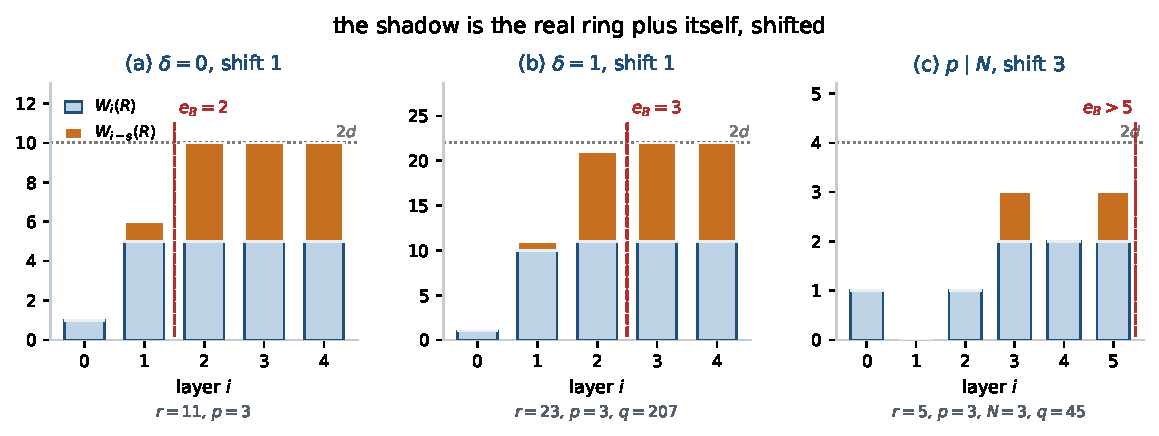
\includegraphics[width=\textwidth]{fig_puente.pdf}
\caption{Theorem~\ref{obs:puente} as an arithmetic of bars: the pale bar is $W_i(R)$, the dark one
is the same bar moved $P$ places to the right, and the total height is $W_i(B)$. The dotted line is
the full dimension $2d$; the conductor exponent of the shadow is the first layer from which the two
bars together reach it, which is $P$ more than for $R$ alone --- that is $e_B=e_R+P$, seen rather
than believed. (a) the generic case. (b) the first conductor where $h^-$ bites, $r=23$ at $p=3$:
the real ring loses one dimension in layer $1$, the shadow loses it twice, one layer apart, and
the conductor goes from the square of the radical to its cube. (c) when $p\mid N$ the shift is
$P=p^{v_p(N)}$ and the pale bar has the ladder shape of Theorem~\ref{thm:escalera}; here the window
stops at $K=6$ before the bars fill, so the mark is a bound and not a value.}
\label{fig:puente}
\end{figure}

\begin{proposition}[the type crosses the bridge]\label{prop:tipopuente}
Under the hypotheses of Theorem~\ref{obs:puente}, $\operatorname{type}(B)=\operatorname{type}(R)$.
If moreover $p\nmid N$ and $d/2<u<d$, then $\operatorname{type}(B)=\delta+\kappa-1$ with $\kappa$
as in \cite[Prop.~11]{Cond}; in particular $B$ is Gorenstein exactly when $\delta=\kappa=1$,
although its conductor is one power ($P=1$) deeper than that of $R$.
\end{proposition}

\begin{proof}
$B$ is free, hence flat, over the local ring $R$, and $\theta^2$ lies in the maximal ideal of $R$
because it has valuation $2P\ge2$, so the closed fibre is $\FF_p[T]/(T^2)$, which is Gorenstein of type
$1$. For a flat local homomorphism with Gorenstein closed fibre the canonical module is the base
change of the canonical module, so the type is multiplied by that of the fibre \cite[\S3.3]{BH}; the residue fields
agree. The second statement is \cite[Prop.~11]{Cond} applied to $R$, which has $e_R=2$ there: with
$p\nmid N$ one has $W_1(R)=u$, and $d/2<u<d$ is the hypothesis of that proposition.
\end{proof}

A conductor that is the square of the radical does not make $R$ Gorenstein. With
$\ell(\cO_+/R)=\sum_{i<e}(d-W_i)$ and $\ell(R/\mathfrak f_R)=\sum_{i<e}W_i$, the Gorenstein
condition $\ell(\cO_+/R)=\ell(R/\mathfrak f_R)$ reads $\sum_{i<e}W_i=ed/2$, which is a separate
condition.

\medido{At $r=41$, $p=11$, $q=451$, $N=1$ the real profile is $(1,18,20,20)$, so $e_R=2$ and the
real conductor is the square of the radical, while $\ell(\cO_+/R)=21\neq19=\ell(R/\mathfrak f_R)$:
$R$ is not Gorenstein, and by Proposition~\ref{prop:tipopuente} neither is $B$, whose conductor is
the cube.}

\medskip
\begin{center}\small
\rowcolors{2}{filaclara}{white}
\begin{tabular}{@{}lllcrr@{}}
\toprule
 & $W(R)$ & $W(B)$ & $e_R\to e_B$ & $v_p([\cO_+:R])$ & $v_p([\cO:B])$ \\
\midrule
$\delta=0$ & $(1,d,d,\dots)$ & $(1,d{+}1,2d,2d,\dots)$ & $1\to2$ & $d-1$ & $3d-2$ \\
$\delta>0$ & $(1,d{-}\delta,d,\dots)$ & $(1,d{+}1{-}\delta,2d{-}\delta,2d,\dots)$ & $2\to3$ &
  $2d-1-u$ & $3d-2+2\delta$ \\
\midrule
$q=207$, $p=3$ & $(1,10,11,\dots)$ & $(1,11,21,22,\dots)$ & $2\to3$ & $11$ & $33$ \\
$q=279$, $p=3$ & $(1,14,15,\dots)$ & $(1,15,29,30,\dots)$ & $2\to3$ & $15^\dagger$ & $45^\dagger$ \\
\bottomrule
\end{tabular}
\end{center}

\noindent{\small The bridge in two regimes and in the only two cells of the swept range with
$\delta>0$, both $r$ prime with $p=3\mid h^-$ and $\delta=1$. The layers are measured; the two
indices at $q=207$ are closed integer lattices, and the two marked $\dagger$ are the law applied to
the measured layers, not lattices. At $q=207$ the plane of \S\ref{sec:loc} would give $32$.}
\medskip

\medido{Independent checks: the displayed identities hold in $306$ of $306$ cells read to depth $K=\min(E,4)$, the index law in
$13$ of $13$ cells by closing integer lattices rather than layers, and the seven steps of the proof
--- the representative, the unit, $\mu\in B$, $B=A[\mu]$, $R=A$, $B^-=\theta R$ and
$v_p(\theta)=P$ --- each separately in $66$ of $66$ cells with integer lattices localised at $p$,
at $P=1$, $3$ and $9$, with $\varphi(p^v)=2$, with composite $r$ and with $N\le9$. Each of the
seven is covered by the proof.}

Three remarks on what the proof does \emph{not} use. It does not need $E\ge3$: nothing is expanded
to second order in $\pi$. Neither it nor Proposition~\ref{prop:tau} needs $u>d/2$; that hypothesis
enters only through what \cite{Cond} can say about the profile of the real
ring, which is what pins $e_R\le2$ and hence the display. And it does not name a symplectic
ring: $R$ is the ring of the centred segment, and the identification of that ring with
$A_{\Sp(2m)}(q)$ for a suitable $m$ is Proposition~\ref{prop:ops} and Corollary~\ref{cor:par}
applied to $S-Nr/2$, whose length is $Nr\pm1$ --- so $m$ depends on $N$, and the naive guess
$m=r-1$ is wrong even locally: at $q=45$, $p=3$, $N=3$ the ring $R$ has $v_3([\cO_+:R])=4$ and
$W_1(R)=0$, while $A_{\Sp(8)}(45)$ has $v_3=1$ and $W_1=2$. Over $9$ cells and $54$ comparisons $A_{\Sp(2m)}(q)$ with
$m=r-1$, $m=r$ and $m=(q-r-2)/2$ give the same truncated image while $m=r-2$ and $m=r+1$ do not, and $m=r-3$ does only in the
two cells at $q=45$, and
the integer lattices of the three are already distinct at $q=45$, of indices $75$, $3$ and $3$.

What the shift measures is the degree of the anti-invariant generator, and that degree has a
reading of its own. Write $n'$ for whichever of $n$, $n-1$ is divisible by $r$; then
$P=v_p(\zeta_q^{\,n'}-1)$ is how far the segment is from closing into a full period. When it does
close, $\zeta_q^{\,n'}=1$ and the extension degenerates --- which is the other thing this section
already knew, $B_n(q)=\ZZ$ at $n\equiv0,1\pmod q$. One number governs both ends.

The shape of Theorem~\ref{obs:puente} is not new: whether an order in a CM field is free of rank
two over the subring fixed by complex conjugation is a hypothesis Howe isolated and used
\cite[pp.~13, 20]{Howe}, and, in the quartic CM setting of \cite{IT}, when the real ring is the \emph{maximal} one the
conductor of such an extension is computed and the order is Gorenstein because it is monogenic
\cite[Lemmas 7, 8]{IT} --- a precedent of shape, not a proof for cyclotomic orders of arbitrary
degree. The graded consequence has a standard shape too: for Artinian graded algebras, $\gr(B)$ over
$\gr(R)$ with fibre $\FF_p[\bar\theta]/(\bar\theta^2)$ is a \emph{free extension} in the sense of
Harima and Watanabe, whose Hilbert function multiplies \cite[Def.~1.5, Lem.~1.6]{IM}. Our graded
rings are not Artinian, so we cite this as context: here the product of Hilbert series is proved
by the filtered direct sum in the proof above, not by \cite{IM}. What is new is which orders these are, and that the real one is not maximal:
there the layers of $R$ are not all full and the convolution has content.

\frontera{\textbf{Where it does break.} Not at $p\mid N$: nothing in the proof looks at $N$
modulo $p$, and the only thing that changes there is the value of $P$. It breaks at $p=2$: the modulus $q$ is even and $2^{-1}$ does not exist modulo $q$. The centring
element may still exist when $Nr$ is even --- $q=20$, $r=5$, $N=2$ has $\mu=\zeta_{20}^{\,5}$ ---
but the proof recovers $\mu$ from $\mu^2$ through its odd order and splits $B$ with the projectors
$(1\pm\iota)/2$, and both steps divide by $2$. That is a different problem, not a harder case of this one --- the
index $2^7$ at $(n,q)=(7,14)$, recorded and unexplained after Theorem~\ref{thm:sombra}, is its
smallest instance. For $u\le d/2$ the ring is still $A$, by Proposition~\ref{prop:tau}, but \cite{Cond} does not
give the profile of $A$ there, so the displayed $W(B)$ does not follow. That is a gap in the real
input, not in the bridge.}

\section{Two frontiers}

\frontera{\textbf{The $h^-$ criterion in the shadow, outside the bridge.} At $q'=31$ with $n=q'$
the real defect is $3$ while the shadow drops by $1$: the two are not compared against the same
ring. Theorem~\ref{obs:puente} says which real ring the shadow is to be compared with --- not the
one of the same $n$, but the one of the segment recentred at $Nr/2$, whose defect there is also
$1$ --- and that is what dissolves the asymmetry inside the main family. What is open is outside
it. When $p\mid N$ --- the second source of defect already present in type $C$ --- the proof does
\emph{not} stop: $e_1(S)$ stays a unit, the residue $\pm1$ coming from the sum over all classes and
not from $N$, and the only thing that changes is that the shift becomes $p^{v_p(N)}$. What is open
there is narrower, and it is not a step: the fixed ring $B^\iota$ is $A$ by
Proposition~\ref{prop:tau}, the ring of the centred segment $S-Nr/2$, which \S\ref{sec:seg}
identifies with a symplectic ring; below depth $P$ that ring follows the ladder
(Theorem~\ref{thm:escalera}), and what is not settled when $p\mid N$ is its profile beyond it. For the shadow's first
layer the question does not arise: Proposition~\ref{prop:capa1} answers it directly, and the answer
is $W_1=0$. And $p=2$ is
a different problem: $q$ is even, $2^{-1}$ does not exist modulo $q$, and even where a centring
element exists the proof's recovery of $\mu$ from $\mu^2$ and its projectors divide by $2$. The statement must be made family by family, as in \cite{Cond}, and not in one
piece.}

\frontera{\textbf{The stratified reading, and the guess it kills.} The columns are permuted by the
strata $X_D=\{c:\gcd(c,q')=D\}\cong(\ZZ/(q'/D))^\times$, which is the structure of
\emph{gcd-graphs}, whose eigenvalues are Ramanujan sums and which by So's theorem are the only
integral circulant graphs \cite{So,KS}. Writing $S_D$ for the restriction of $S$ to $X_D$, the
annihilator splits, $\operatorname{Ann}(S)=\bigcap_D\operatorname{Ann}(S_D)$, so
\[
\marco{W_1=\operatorname{codim}_{\FF_p[G]}\ \bigcap_{D\mid q'}\operatorname{Ann}(S_D),\qquad
G=(\ZZ/q')^\times,}
\]
which is the stratified reading in its correct form: when $p\nmid\varphi(q')$ the group algebra is
semisimple and a block counts once, as soon as it survives in \emph{at least one} stratum. Summing
the strata instead counts it once per stratum, which is why that overshoots.
What does not work is the refinement one wants next. A character of conductor $f$ appears in every
stratum with $f\mid q'/D$, so one hopes it either survives in all of them or in none, which would
make $\operatorname{codim}\operatorname{Ann}(S_D)$ a divisor sum in $q'/D$ and give a count by
conductor. It is false: survival depends on the stratum, and in $76$ of $416$ stable cells even the
unit stratum $D=1$, the largest, fails to see the whole first layer. A witness with a semisimple
group algebra is in the shadow, the segment $\{0,\dots,13\}$ of $\GL(14)$ at $q'=14$, $p=5$
($q=70$, and $5\nmid\varphi(14)$), where the layer dimension is $\varphi(14)=6$, $W_1=4$
and $\operatorname{codim}\operatorname{Ann}(S_1)=3$: a block dies on the units and lives on a
smaller stratum. So a count by conductor that assumes a block survives uniformly across the strata
is false; a classification by conductor that carries the data of the strata is not ruled out, and
what is missing is a description of which strata a block survives in.}

\begin{remark}[a negative result]
$\gr_1(A)$ is \emph{not} the Galois orbit of a single element of $\bar R$: it is the span of all the
coefficients of one polynomial. Three attempts to describe it as such --- the module generated by
$\sum_cS(c)\omega^c$, the sum of the ranks stratum by stratum, and the module generated by
$\sum_cS(c)U_c\omega^c$ --- give $181$, $169$ and $101$ of the $193$ stable cells, against $193$ for
the matrix of Theorem~\ref{thm:loc}.
\end{remark}

\section{What this computes, and a tool that computes it}\label{sec:util}

Two of the statements above replace a computation by a formula, and that is worth saying in the
currency of whoever has to do the computation. The object is an order in a cyclotomic field and the
question is its conductor; that is the everyday task in the algorithmics of complex multiplication,
where the conductor of a CM order is what one computes in order to identify an endomorphism ring or
to place a curve in an isogeny graph \cite{IT,BSt13}. In that setting the two read as follows.

\emph{A filter that costs nothing.} Theorem~\ref{thm:sop} says that $p$ can divide $[\cO:A]$ only
when $r$ divides one of $n-1,n,n+1$, and Corollary~\ref{cor:sopsombra} narrows that to $n,n-1$ for
the shadow. That is a divisibility test: no lattice, no matrix, no layers. It certifies maximality at
every prime outside the families in the time it takes to reduce $n$ modulo $r$, and it can be run over as many pairs as one likes before any real work starts.

\emph{Half the degree.} Theorem~\ref{obs:puente} gives
$v_p([\cO:B_n])=2\,v_p([\cO_+:R])+P\,d$. The left side is an invariant of an order of degree
$\varphi(q)$; the right side is computed in the real subfield, of degree $\varphi(q)/2$, plus one
multiplication. This is the shape of statement that the CM literature has for the case where the
real order is \emph{maximal} \cite[Lemmas 7, 8]{IT}; what is new is that it does not need that.

The tool also implements, as \texttt{ceros} and \texttt{fila}, the two counts of the companion
note \cite{II}: the vanishing components on the diagonal, and the rows a quadratic character
occupies --- exactly those with $\bigl(\frac2n\bigr)=1$, which \cite{II} proves by showing that a
completely multiplicative sign pattern with zero weighted sum exists at every admissible length.

\paragraph{The tool.} \texttt{segmento.py} travels with this note: one file, Python~3 standard
library only, no installation and no computer algebra system. It exposes
\texttt{familias}, \texttt{perfil}, \texttt{indice}, \texttt{puente}, \texttt{ceros} and
\texttt{fila} --- one routine per statement of this note and of \cite{II}, named after it --- as a
library and as a command line, together with \texttt{segmento\_SU}, which returns the segment of
$g_q$ with its modulus ($M=2q$ for $n$ even, as in \S\ref{sec:seg}). Running \texttt{python segmento.py autotest} reproduces, from
scratch, the worked examples of this note --- the profiles $(1,11,21,22)$ at $q=207$ and
$(1,15,29,30)$ at $q=279$, the index $v_3([\cO:B_{23}(207)])=33$ --- and those of \cite{II}. The slow
path, \texttt{indice}, is kept deliberately: it is the control against which the formulas are
checked, and the check is part of the test. It is also deposited on its own, under CC0 and with a
DOI of its own \cite{Tool}, so that it can be found, used and cited by someone who never reads this
note --- which is the audience an application has.

\medido{The shortcut against the slow path in $9$ cells with $\varphi(q)\le132$: the same integer
in every cell, and about half the wall clock at the largest of them. The factor is the ratio of the
two degrees and not an asymptotic claim --- both routes run the same layer code, and the only
difference is that one closes in degree $\varphi(q)$ and the other in $\varphi(q)/2$; the times
themselves are a property of the machine and the archived run records them. The script that times
it, \texttt{medir\_atajo.py}, travels with the note as well.}

\noindent What the tool does \emph{not} do is hide the honesty floor of the note: where a
statement is measured and not proved --- the count of vanishing components at a composite $f$,
where that count needs $f$ prime --- the corresponding routine says so and declines; and where the layer profile is cut at depth $E$
before it fills, \texttt{indice} and \texttt{puente} return a lower bound and say so; and at
$q'\le2$, outside Theorem~\ref{thm:loc}, \texttt{indice} declines. The guards are exactly these
three and no others. The shortcut is not guarded at $u\le d/2$, because
Proposition~\ref{prop:tau} gives $R=A$ unconditionally; and it is not guarded at $p\mid N$,
and should not be, because there the number is justified and what stays open is the deeper
profile of the real side, not a step.

\section*{MSC 2020}
Primary 11R18; Secondary 11R29, 11R04, 13H10, 13B22, 05C50, 20G05, 11Y40.

\section*{Declaration of competing interest}
The author declares no competing interest and no funding.

\section*{Data availability}
No external data were used. The computational data --- every number labelled \emph{measured}, and
every figure --- are generated by scripts that travel with this note together with their archived
output. Among them is \texttt{segmento.py} of \S\ref{sec:util}, a single dependency-free file that
implements the statements of this note and verifies its own numbers with
\texttt{python segmento.py autotest}; it is released into the public domain under CC0 so that it
can be used, cut up or rewritten without asking, and is deposited as a citable software record of
its own \cite{Tool}.

\section*{Declaration on generative AI}
This note was written with Claude (Anthropic) as an assistant, under the author's direction. Every
statement marked \emph{measured} is produced by a script archived with the note; the author is
responsible for the content.

\begin{thebibliography}{99}
\bibitem{BS} A.~B\"achle, B.~Sambale, \emph{Orders generated by character values},
Monatsh.~Math.~\textbf{191} (2020), 665--678.
\bibitem{BSt13} G.~Bisson, M.~Streng, \emph{On polarised class groups of orders in quartic
CM-fields}, Math.~Proc.~Cambridge Philos.~Soc.~\textbf{163} (2017), 233--254,
\href{https://arxiv.org/abs/1302.3756}{\texttt{arXiv:1302.3756}}.

\bibitem{CMP} P.~Cellini, P.~M\"oseneder Frajria, P.~Papi, \emph{The $\widehat W$-orbit of $\rho$,
Kostant's formula for powers of the Euler product and affine Weyl groups as permutations of
$\mathbb{Z}$}, J.~Pure Appl.~Algebra \textbf{208} (2007), 1103--1119;
\texttt{arXiv:math/0507610}.
\bibitem{Ded77} R.~Dedekind, \emph{\"Uber die Anzahl der Ideal-Klassen in den verschiedenen Ordnungen
eines endlichen K\"orpers}, Festschrift der Technischen Hochschule Braunschweig, Vieweg (1877),
1--55.
\bibitem{FSS} J.~Fuchs, A.~N.~Schellekens, C.~Schweigert, \emph{From Dynkin diagram symmetries to
fixed point structures}, Comm.~Math.~Phys.~\textbf{180} (1996), 39--97.
\bibitem{Hopper} J.~Hopper, \emph{The twining character formula for reductive groups},
\texttt{arXiv:2204.03600}.
\bibitem{Jan} J.~C.~Jantzen, \emph{Darstellungen halbeinfacher Gruppen und kontravariante Formen},
J.~reine angew.~Math.~\textbf{290} (1977); the twining character formula goes back to his 1973 work.
\bibitem{Howe} E.~W.~Howe, \emph{Kernels of polarizations of abelian varieties over finite fields},
J.~Algebraic Geom.~\textbf{5} (1996), 583--608; page numbers as in the reproduction of the 1995
preprint, \href{https://arxiv.org/abs/2001.05111}{\texttt{arXiv:2001.05111}}.

\bibitem{IM} A.~Iarrobino, P.~Macias Marques, C.~McDaniel, \emph{Artinian Gorenstein algebras that
are free extensions
over $k[t]/(t^n)$, and Macaulay duality}, J.~Pure Appl.~Algebra \textbf{224} (2020), 106305,
\href{https://arxiv.org/abs/1807.02881}{\texttt{arXiv:1807.02881}}; free extensions are due to
T.~Harima and J.~Watanabe.

\bibitem{IT} S.~Ionica, E.~Thom\'e, \emph{Isogeny graphs with maximal real multiplication},
J.~Number Theory \textbf{207} (2020), 385--422,
\href{https://arxiv.org/abs/1407.6672}{\texttt{arXiv:1407.6672}}; Lemma~7 is due to E.~Goren and
K.~Lauter, and Lemma~8 rests on J.~Buchmann and H.~W.~Lenstra, \emph{Approximating rings of
integers in number fields}, J.~Th\'eor.~Nombres Bordeaux \textbf{6} (1994), 221--260, (2.7)--(2.8).

\bibitem{KS} W.~Klotz, T.~Sander, \emph{Some properties of unitary Cayley graphs},
Electron.~J.~Combin.~\textbf{14} (2007).
\bibitem{Kostant76} B.~Kostant, \emph{On Macdonald's $\eta$-function formula, the Laplacian and
generalized exponents}, Adv.~Math.~\textbf{20} (1976), 179--212.
\bibitem{Kostant04} B.~Kostant, \emph{Powers of the Euler product and commutative subalgebras of a
complex simple Lie algebra}, Invent.~Math.~\textbf{158} (2004), 181--226.
\bibitem{Cond} C.~Mar\'in, \emph{Where the character values of $\Sp(2m)$ at a torsion element fail
to generate the ring of integers}, \href{https://doi.org/10.5281/zenodo.22813216}{\texttt{doi:10.5281/zenodo.22813216}}, 2026.
\bibitem{Tool} C.~Mar\'in, \emph{Computing the conductor and index of orders generated by
character values: an exact, dependency-free Python tool for $\SU(n)$, $\Sp(2m)$ and $\GL(n)$
(\texttt{segmento.py})}, software, v1.0.0, CC0,
\href{https://doi.org/10.5281/zenodo.22834098}{\texttt{doi:10.5281/zenodo.22834098}}, 2026.
\bibitem{Des82} J.~D\'esarm\'enien, \emph{Un analogue des congruences de Kummer pour les
$q$-nombres d'Euler}, European J.~Combin.~\textbf{3} (1982), 19--28.

\bibitem{Oli65} G.~Olive, \emph{Generalized powers}, Amer.~Math.~Monthly \textbf{72} (1965),
619--627.

\bibitem{Sag92} B.~E.~Sagan, \emph{Congruence properties of $q$-analogs}, Adv.~Math.~\textbf{95}
(1992), 127--143; the $q$-Lucas theorem is Theorem~2.2, with its history on p.~131.

\bibitem{NS07} S.~G.~Naculich, H.~J.~Schnitzer, \emph{Level-rank duality of the $U(N)$ WZW model,
Chern--Simons theory, and 2d qYM theory}, JHEP \textbf{0706} (2007) 023,
\href{https://arxiv.org/abs/hep-th/0703089}{\texttt{arXiv:hep-th/0703089}}.

\bibitem{NT92} T.~Nakanishi, A.~Tsuchiya, \emph{Level-rank duality of WZW models in conformal field
theory}, Comm.~Math.~Phys.~\textbf{144} (1992), 351--372.

\bibitem{ABI90} D.~Altschuler, M.~Bauer, C.~Itzykson, \emph{The branching rules of conformal
embeddings}, Comm.~Math.~Phys.~\textbf{132} (1990), 349--364.

\bibitem{SA91} H.~Saleur, D.~Altschuler, \emph{Level-rank duality in quantum groups},
Nucl.~Phys.~B \textbf{354} (1991), 579--613.

\bibitem{MNRS91} E.~J.~Mlawer, S.~G.~Naculich, H.~A.~Riggs, H.~J.~Schnitzer, \emph{Group-level
duality of WZW fusion coefficients and Chern--Simons link observables}, Nucl.~Phys.~B \textbf{352}
(1991), 863--896.

\bibitem{Fre82} I.~B.~Frenkel, \emph{Representations of affine Lie algebras, Hecke modular forms and
Korteweg--de Vries equations}, in Lie Algebras and Related Topics, Lecture Notes in
Math.~\textbf{933}, Springer, 1982, p.~71.

\bibitem{BH} W.~Bruns, J.~Herzog, \emph{Cohen--Macaulay Rings}, rev.~ed., Cambridge Stud.~Adv.~Math.
\textbf{39}, Cambridge Univ.~Press, 1998.

\bibitem{PS86} A.~Pressley, G.~Segal, \emph{Loop Groups}, Oxford Univ.~Press, 1986; the
$k\leftrightarrow N-k$ symmetry is Proposition~(10.6.4), p.~212, as cited in \cite{Wit93}.

\bibitem{Wit93} E.~Witten, \emph{The Verlinde algebra and the cohomology of the Grassmannian},
\href{https://arxiv.org/abs/hep-th/9312104}{\texttt{arXiv:hep-th/9312104}}; in Geometry, Topology
and Physics, Conf.~Proc.~Lecture Notes Geom.~Topology IV, Int.~Press, 1995, 357--422.

\bibitem{NPP} S.~Nadimpalli, S.~Pattanayak, D.~Prasad, \emph{Character theory at a torsion element},
\texttt{arXiv:2504.14684}.
\bibitem{Pia87} A.~Pianzola, \emph{On the arithmetic of the representation ring and elements of
finite order in Lie groups}, J.~Algebra \textbf{108} (1987), 1--33.
\bibitem{Sin78} W.~Sinnott, \emph{On the Stickelberger ideal and the circular units of a cyclotomic
field}, Ann.~of Math.~\textbf{108} (1978), 107--134.
\bibitem{So} W.~So, \emph{Integral circulant graphs}, Discrete Math.~\textbf{306} (2006), 153--158.
\bibitem{II} C.~Mar\'in, \emph{Zeros of weighted partial sums of completely multiplicative
functions: Dirichlet characters, the Euler factor at $2$ and Conrey's sine series},
\href{https://doi.org/10.5281/zenodo.22847374}{\texttt{doi:10.5281/zenodo.22847374}}, 2026.

\end{thebibliography}

\end{document}
